\documentclass{../common/SCNU_Experimental_Report}

\studentname{汤承洲}
\studentid{20233902058}
\major{电子信息工程}
\class{23级2班}
\coursename{控制工程}
\projectname{控制系统古典分析}
\verify
\experimentdate{2026年5月26日}
\teacher{熊爱民}

\graphicspath{{./figures/}}

\begin{document}
\maketitle

\section{实验目的}
以MATLAB为工具，对控制系统进行时域与频域分析。通过传递函数、零极点模型和状态空间模型三种数学模型的相互转换，掌握系统的不同描述方式；利用step()、impulse()、lsim()等函数求解典型输入信号下的输出响应，分析系统的动态特性；研究二阶系统阻尼比和无阻尼自然频率对阶跃响应的影响，分析零点与稳态值的关系；基于开环频率特性曲线计算幅值裕度和相位裕度，判断闭环稳定性；通过Bode图进行频域稳定性分析，寻找使系统获得最大相位裕度的最优增益；分析非最小相位系统的频域特性；最后利用Smith预估器解决时延系统问题。

\section{实验原理}
\subsection{时域分析法}
时域分析法是根据系统的微分方程（或传递函数），利用拉普拉斯变换直接解出动态方程，并依据过程曲线及表达式分析系统的性能。典型的时域响应指标包括：

\begin{itemize}
    \item 延迟时间 $t_d$：响应曲线第一次达到其终值一半所需的时间。
    \item 上升时间 $t_r$：响应从终值10\%上升到终值90\%所需的时间；对有振荡的系统，也可定义为响应从零第一次上升到终值所需的时间。
    \item 峰值时间 $t_p$：响应超过终值达到第一个峰值所需的时间。
    \item 调节时间 $t_s$：响应达到并保持在终值$\pm5\%$（或$\pm2\%$）内所需的时间。
    \item 超调量 $\sigma\%$：响应的最大偏离量与终值之差的百分比。
    \begin{equation}
    \sigma\% = \frac{h(t_p) - h(\infty)}{h(\infty)} \times 100\%
    \end{equation}
    \item 稳态误差：描述系统稳态性能的指标。
\end{itemize}

\subsection{频域分析法}
频域分析法从频率特性出发对系统进行研究。通常将频率特性绘制成各种曲线，包括幅频特性曲线、相频特性曲线、幅相频率特性曲线（Nyquist图）、对数频率特性曲线（Bode图）等。对于最小相位系统，幅频特性和相频特性之间存在唯一对应关系，根据对数幅频特性可唯一确定相频特性和传递函数。通过系统的开环频率特性可以判断闭环系统的性能，分析系统参数对性能的影响。

幅值裕度（Gain Margin, GM）和相位裕度（Phase Margin, PM）是衡量系统稳定性的重要指标：
\begin{itemize}
    \item 幅值裕度：在相角穿越频率处，系统达到不稳定前所能增加的增益倍数。
    \item 相位裕度：在幅值穿越频率处，系统达到不稳定前所能增加的相位滞后量。
\end{itemize}

\subsection{非最小相位系统}
如果系统在右半平面（RHP）有零点或极点，或者包含时延环节，则称为非最小相位系统。非最小相位系统的相位滞后超过具有相同幅频特性的最小相位系统的相位滞后。

\subsection{Smith预估器}
Smith预估器是一种针对时延系统的控制方法。其核心思想是在控制器内部建立一个被控对象（不含时延）和时延的模型，将时延从闭环特征方程中移除，使控制器可以基于无时延的对象进行设计。

\section{实验内容}

\subsection{Task 1：三种数学模型的转换}
\subsubsection{实验描述}
使用MATLAB将传递函数$G(s) = \dfrac{20}{s^2 + 2s - 3}$分别转换为零极点模型和状态空间模型，并利用tf2ss()函数进行手动转换，比较不同转换方法的结果差异。

\subsubsection{关键代码}
\begin{lstlisting}[language=Matlab, caption=Task 1 核心代码]
s = tf('s');
G_tf = 20/(s^2 + 2*s - 3);
G_zpk = zpk(G_tf);
G_ss = ss(G_tf);
[num, den] = tfdata(G_tf, 'v');
[A, B, C, D] = tf2ss(num, den);
\end{lstlisting}

\subsubsection{关键结果}
\begin{itemize}
    \item 传递函数：$G(s) = \dfrac{20}{s^2 + 2s - 3}$
    \item 零极点模型：$G(s) = \dfrac{20}{(s+3)(s-1)}$
    \item 状态空间模型（ss()函数）：$A = \begin{bmatrix} -2 & 1.5 \\ 2 & 0 \end{bmatrix}$,\; $B = \begin{bmatrix} 4 \\ 0 \end{bmatrix}$,\; $C = \begin{bmatrix} 0 & 2.5 \end{bmatrix}$,\; $D = 0$
    \item tf2ss()函数结果：$A = \begin{bmatrix} -2 & 3 \\ 1 & 0 \end{bmatrix}$,\; $B = \begin{bmatrix} 1 \\ 0 \end{bmatrix}$,\; $C = \begin{bmatrix} 0 & 20 \end{bmatrix}$,\; $D = 0$
\end{itemize}

两种方法得到的状态空间实现形式不同（坐标变换关系），但具有相同的传递函数和系统特性，验证了状态空间表示的非唯一性。

\vspace{1em}
\noindent\textbf{重要结果表格：}
\begin{table}[H]
\centering
\caption{Task 1 模型转换结果对比}
\begin{tabular}{lcc}
\toprule
\textbf{模型类型} & \textbf{函数} & \textbf{结果} \\
\midrule
传递函数 & tf() & $20/(s^2 + 2s - 3)$ \\
零极点模型 & zpk() & $20/[(s+3)(s-1)]$ \\
状态空间（内部） & ss() & $A=[-2,1.5;2,0]$, $B=[4;0]$, $C=[0,2.5]$, $D=0$ \\
状态空间（tf2ss） & tf2ss() & $A=[-2,3;1,0]$, $B=[1;0]$, $C=[0,20]$, $D=0$ \\
\bottomrule
\end{tabular}
\end{table}

\subsection{Task 2：典型输入信号的输出响应}
\subsubsection{实验描述}
给定系统$G(s) = \dfrac{20}{s^2 + 2s + 20}$，分别求解其阶跃响应（step）、脉冲响应（impulse）、斜坡响应和抛物线响应（lsim），并分析系统的初始条件响应。

\subsubsection{关键代码}
\begin{lstlisting}[language=Matlab, caption=Task 2 核心代码]
s = tf('s');
G = 20/(s^2 + 2*s + 20);

% 阶跃响应
step(G);

% 脉冲响应
impulse(G);

% 斜坡响应
u_ramp = t;
[y_ramp, t_out] = lsim(G, u_ramp, t);

% 抛物线响应
u_para = 0.5 * t.^2;
[y_para, t_out] = lsim(G, u_para, t);

% 初始条件响应
[y_ic, t_ic] = initial(ss(G), [1; 0], 10);
\end{lstlisting}

\subsubsection{实验结果}

\begin{figure}[H]
\centering
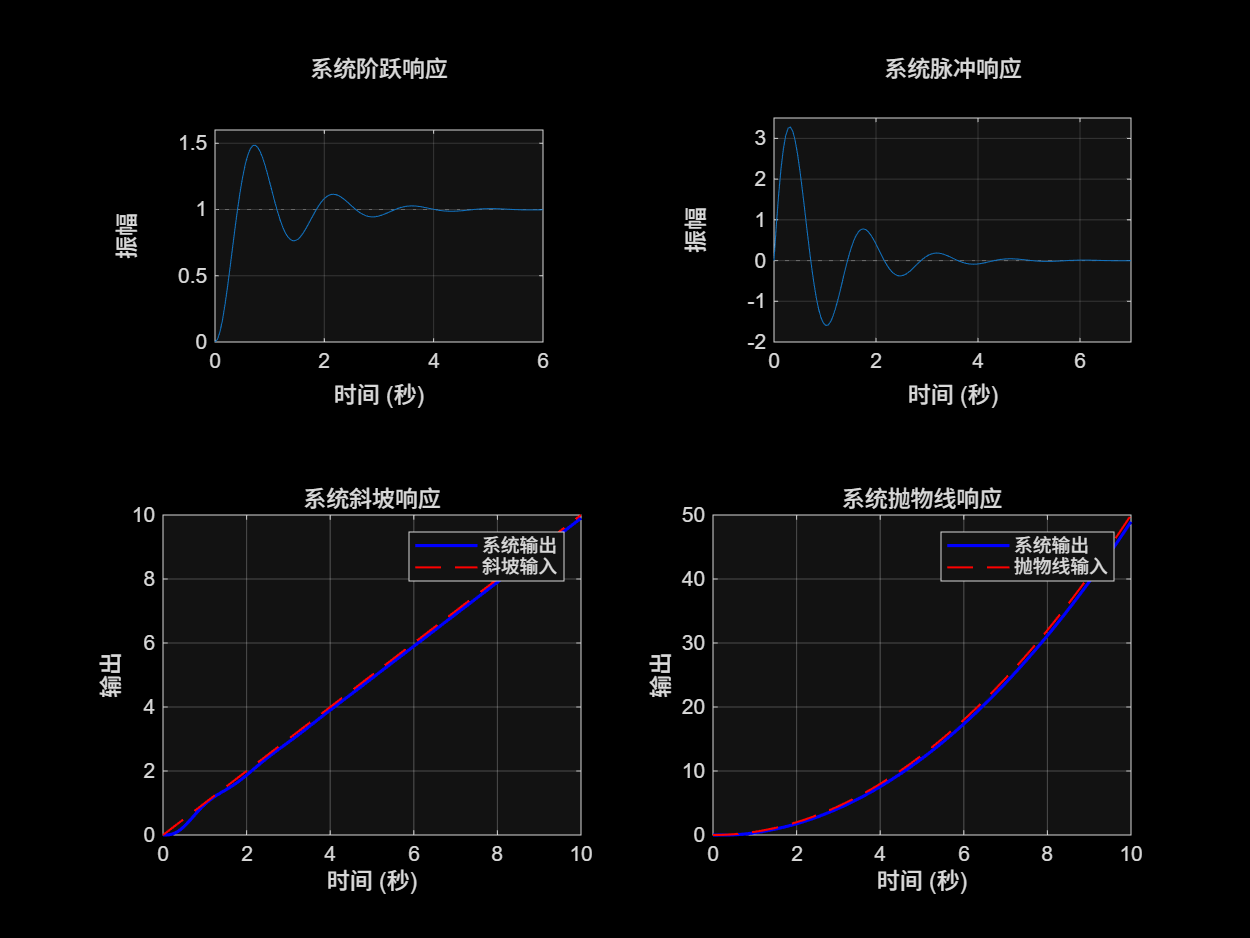
\includegraphics[width=\textwidth]{./figures/Task02_Figure_01.png}
\caption{Task 2 各输入响应（阶跃、脉冲、斜坡、抛物线）}
\end{figure}

\begin{figure}[H]
\centering
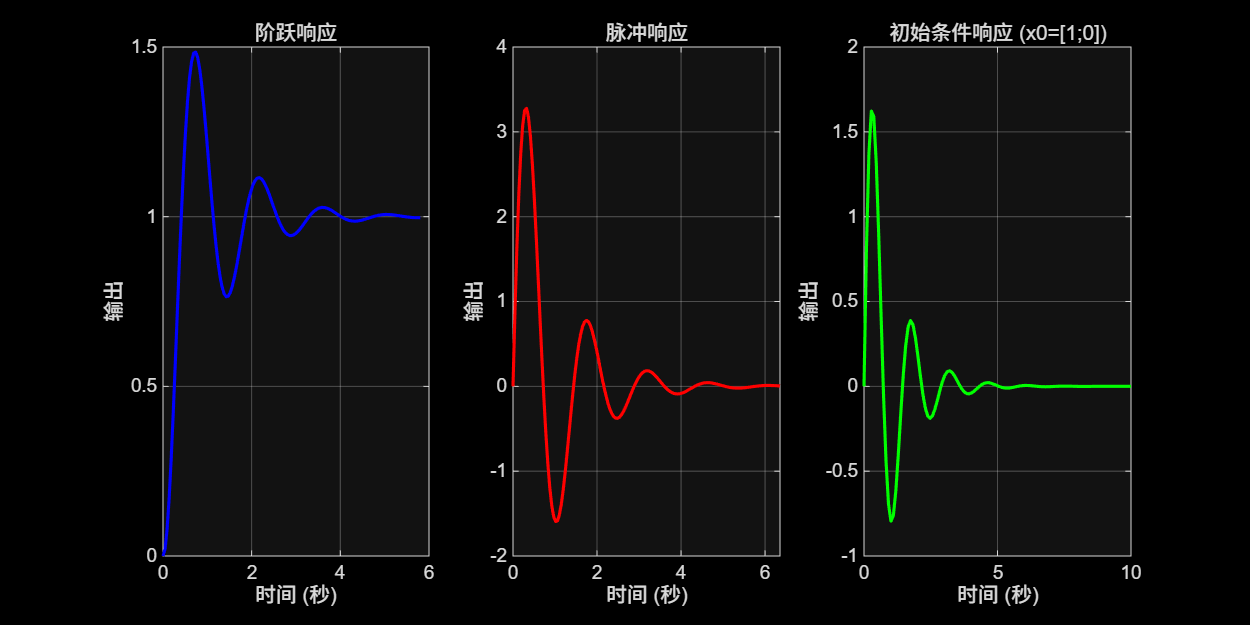
\includegraphics[width=\textwidth]{./figures/Task02_Figure_02.png}
\caption{Task 2 不同输入响应比较（阶跃、脉冲、初始条件响应）}
\end{figure}

\subsubsection{分析}
\begin{itemize}
    \item 阶跃响应反映系统的跟踪能力，系统最终稳态值为1。
    \item 脉冲响应反映系统的动态特性，系统受到瞬时扰动后的恢复能力良好。
    \item 斜坡响应（匀速信号）和抛物线响应（匀加速信号）通过lsim()求解，展示系统对不同输入信号的跟踪能力。
    \item 初始条件响应$x_0=[1;0]^T$表明在没有外部输入时，系统的初始状态如何演化。
\end{itemize}

\subsection{Task 3：二阶系统阶跃响应分析}
\subsubsection{实验描述}
已知二阶系统$G(s) = \dfrac{20}{s^2 + 2s + 20}$，分析阻尼比$\zeta$和无阻尼自然频率$\omega_n$对阶跃响应的影响，并比较$G_1(s)$至$G_4(s)$的响应差异。

\subsubsection{关键代码}
\begin{lstlisting}[language=Matlab, caption=Task 3 核心代码]
% 阻尼比变化
zeta_vals = [zeta_orig, 0.5, 3];
wn_fixed = omega_n_orig;
for i = 1:length(zeta_vals)
    Gi = wn_fixed^2 / (s^2 + 2*zeta_vals(i)*wn_fixed*s + wn_fixed^2);
    [y, t] = step(Gi);
end

% 自然频率变化
omega_n_ref = sqrt(10);
omega_n_vals = [omega_n_ref/3, omega_n_ref, 3*omega_n_ref, omega_n_orig];
z_fixed = zeta_orig;
for i = 1:length(omega_n_vals)
    Gi = omega_n_vals(i)^2 / (s^2 + 2*z_fixed*omega_n_vals(i)*s + omega_n_vals(i)^2);
    [y, t] = step(Gi);
end

% G1-G4阶跃响应比较
G1 = 3*s / (s^2 + 3*s + 10);
G2 = (3*s + 10) / (s^2 + 3*s + 10);
G3 = (s^2 + s) / (s^2 + 3*s + 10);
G4 = (s^2 + s + 10) / (s^2 + 3*s + 10);
\end{lstlisting}

\subsubsection{实验结果}

\begin{figure}[H]
\centering
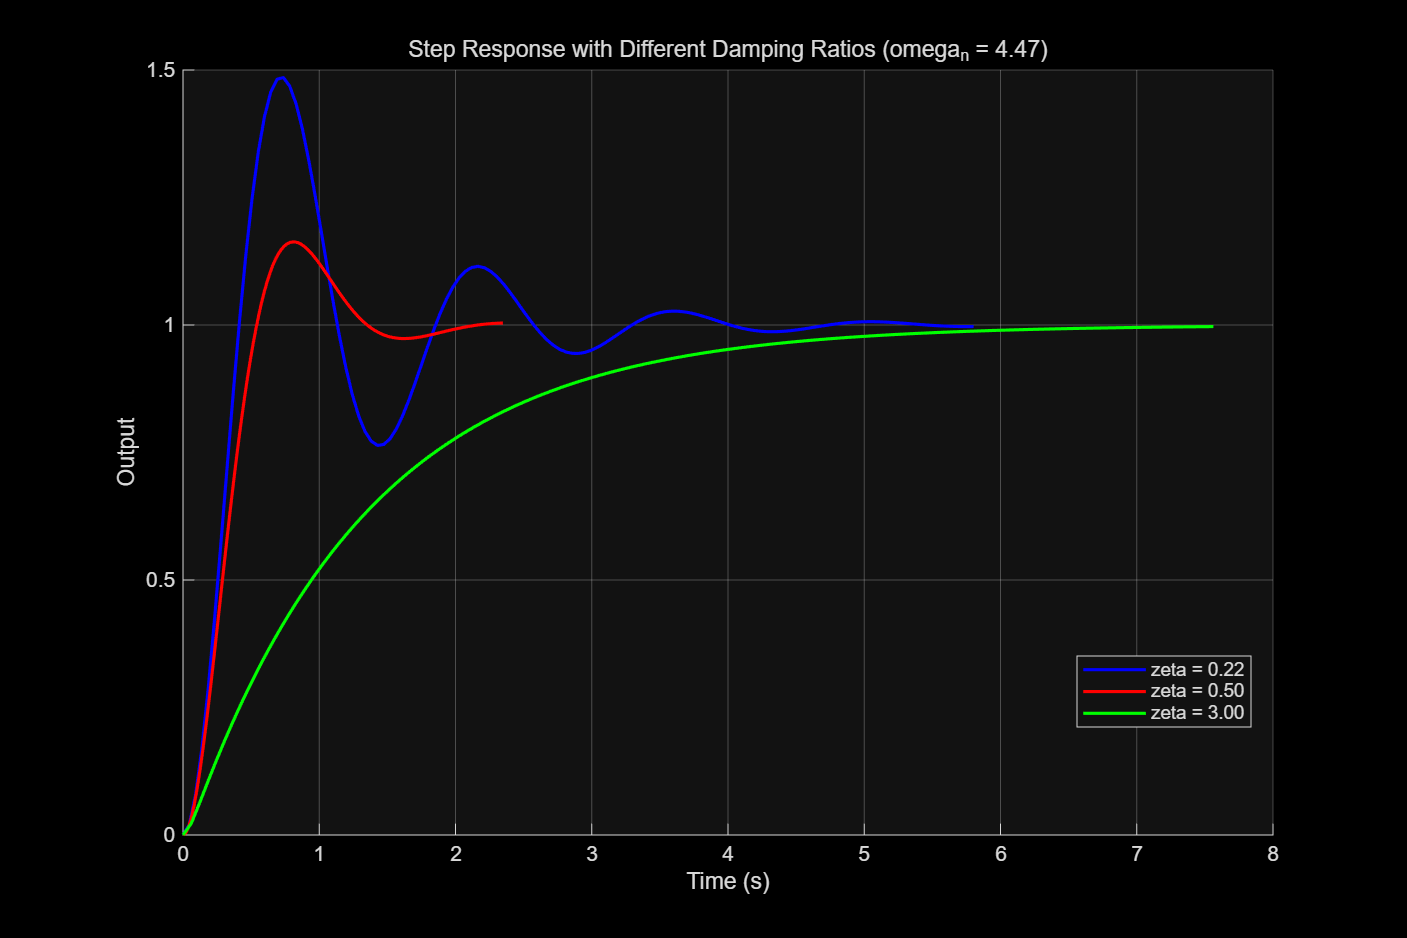
\includegraphics[width=0.85\textwidth]{./figures/Task03_Figure_01.png}
\caption{Task 3(1a)：不同阻尼比下的阶跃响应（$\omega_n = 4.47$固定）}
\end{figure}

\begin{figure}[H]
\centering
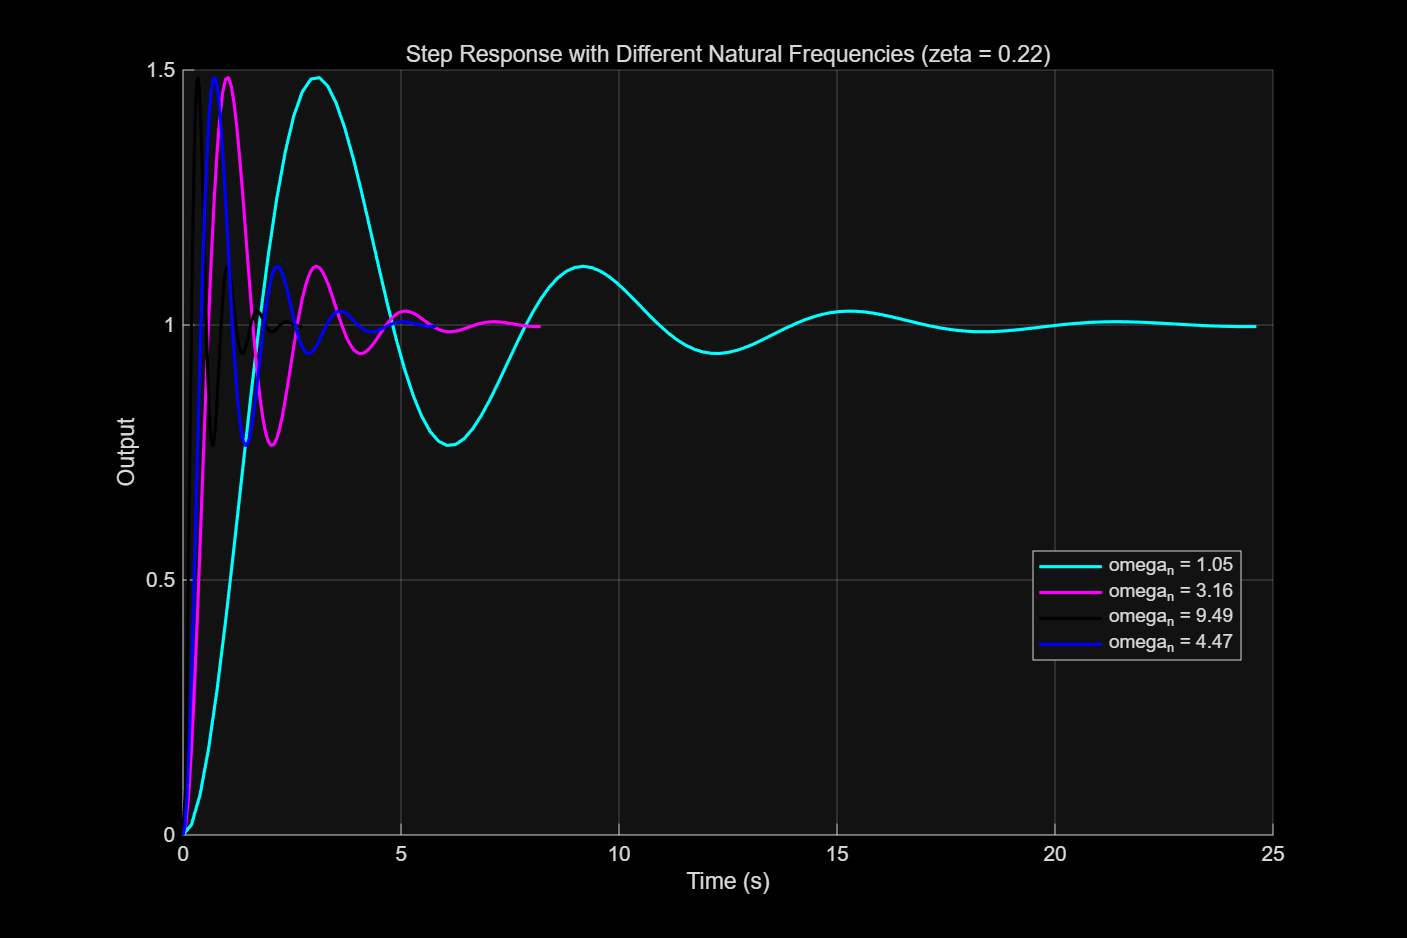
\includegraphics[width=0.85\textwidth]{./figures/Task03_Figure_02.png}
\caption{Task 3(1b)：不同自然频率下的阶跃响应（$\zeta = 0.22$固定）}
\end{figure}

\begin{figure}[H]
\centering
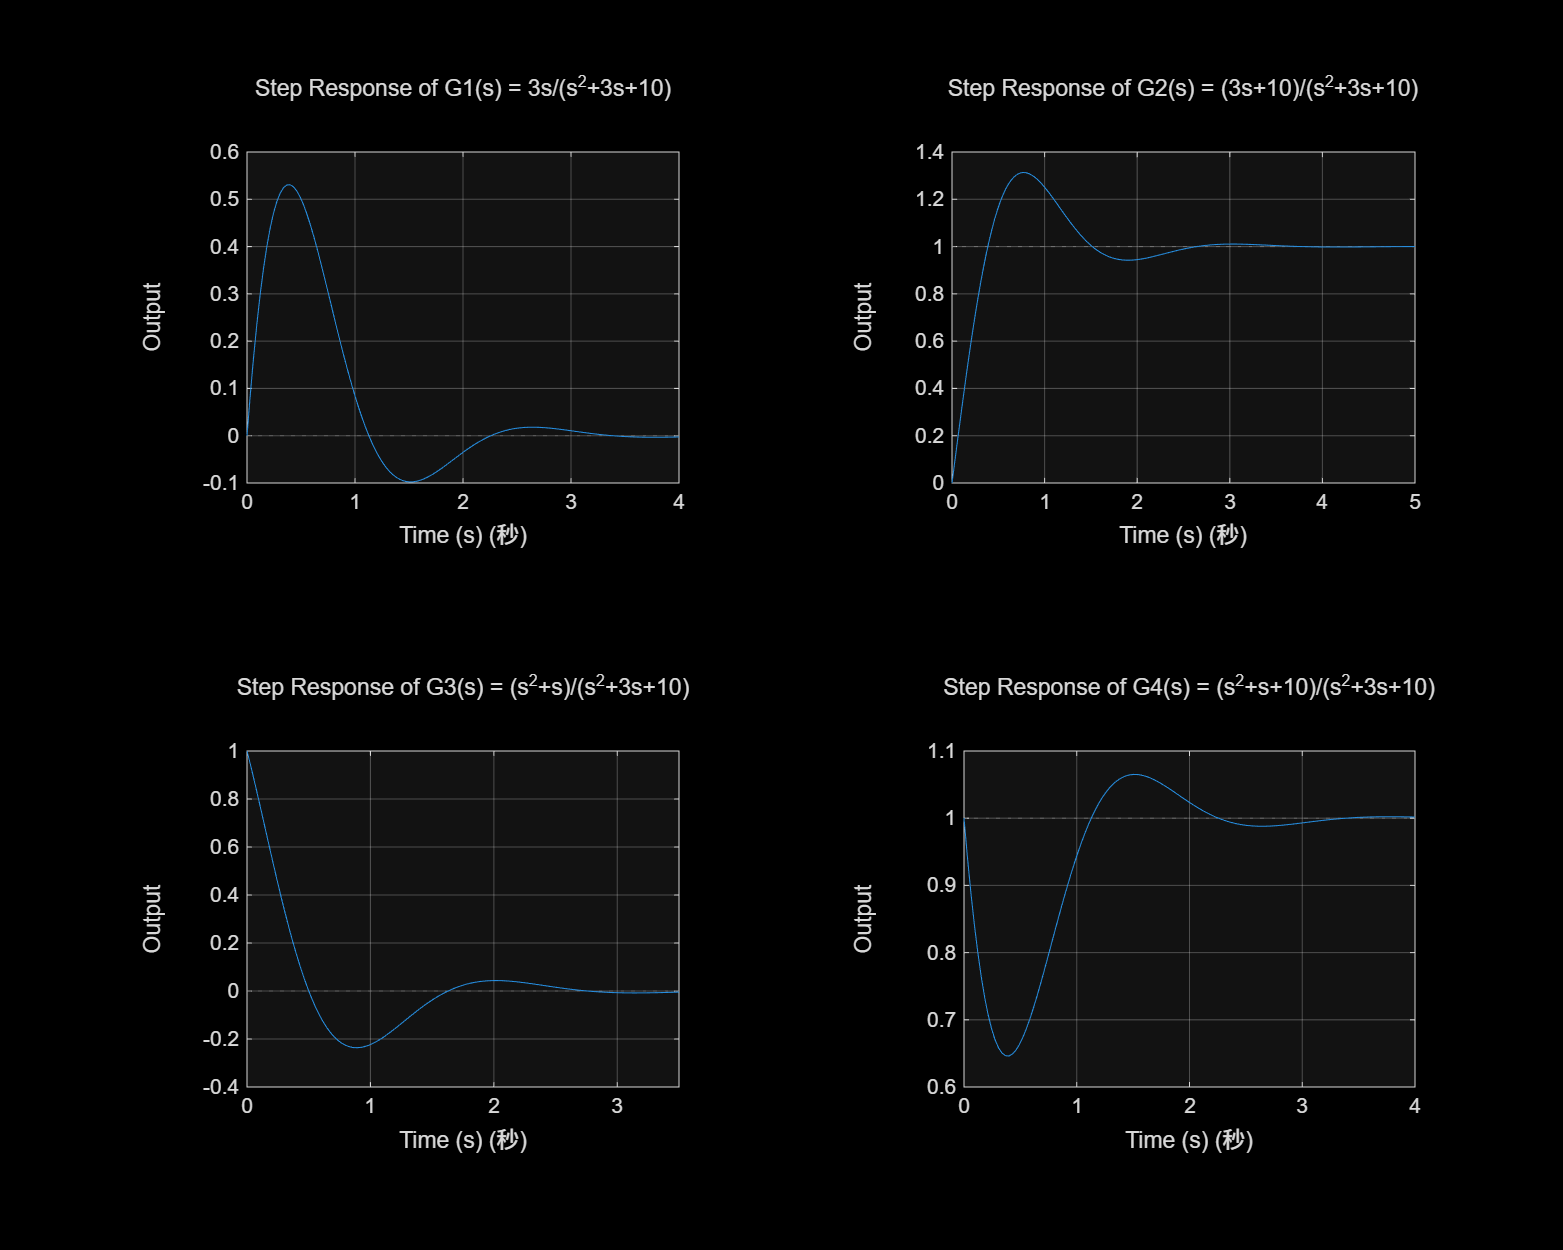
\includegraphics[width=0.85\textwidth]{./figures/Task03_Figure_03.png}
\caption{Task 3(2)：G1--G4的阶跃响应独立子图}
\end{figure}

\begin{figure}[H]
\centering
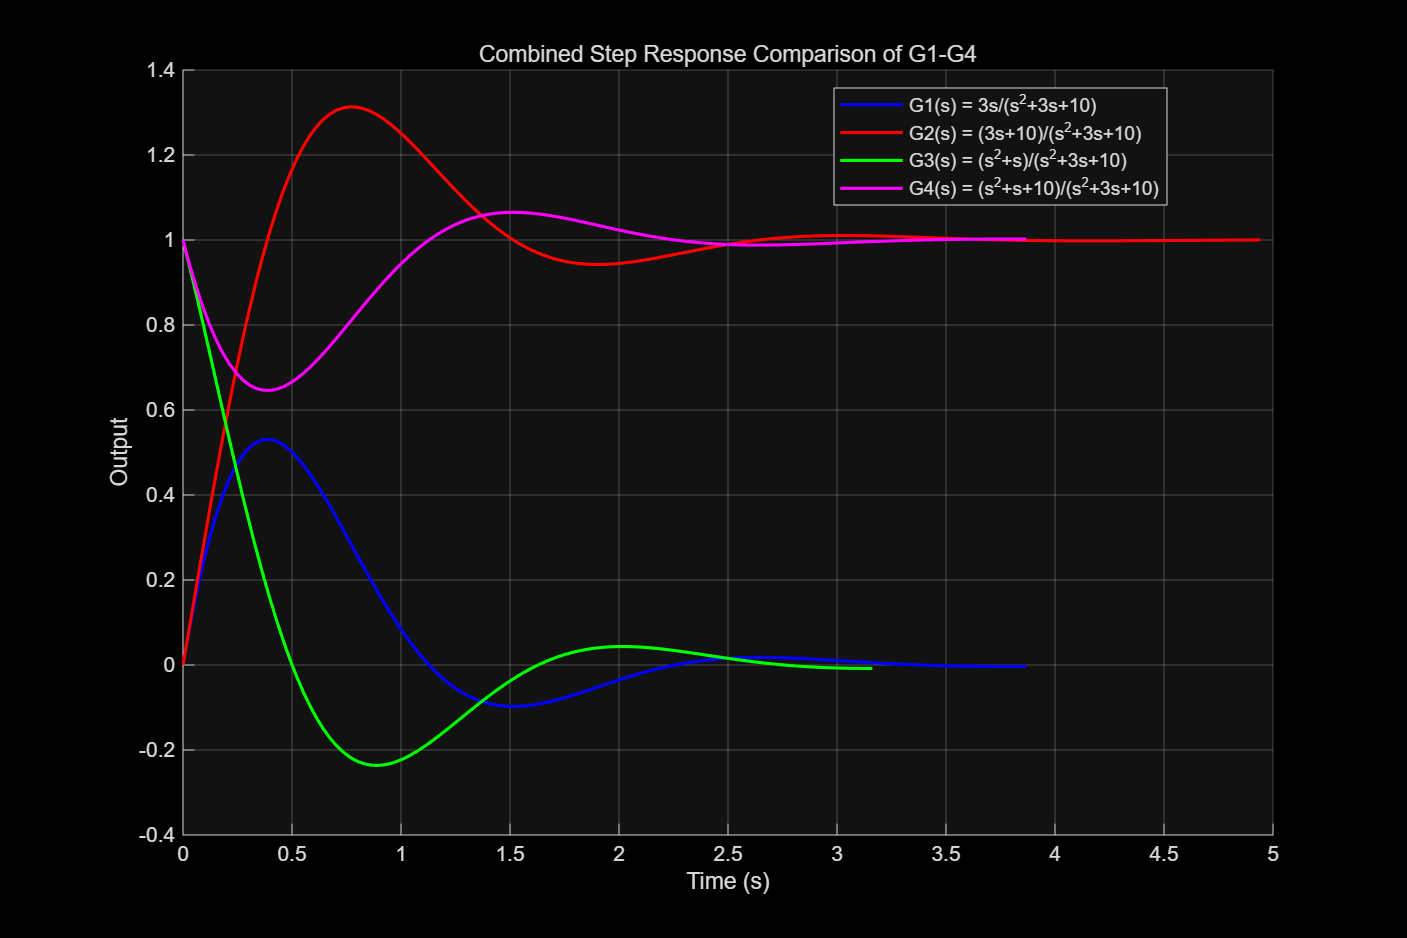
\includegraphics[width=0.85\textwidth]{./figures/Task03_Figure_04.png}
\caption{Task 3(2)：G1--G4的阶跃响应对比}
\end{figure}

\subsubsection{关键结果}
\noindent\textbf{表1：阻尼比对阶跃响应的影响}
\begin{table}[H]
\centering
\caption{不同阻尼比参数对比}
\begin{tabular}{cccc}
\toprule
$\zeta$ & $\omega_n$ & 传递函数 & 响应特征 \\
\midrule
0.22（原系统） & 4.4721 & $20/(s^2 + 2.00s + 20)$ & 欠阻尼，中等超调 \\
0.50 & 4.4721 & $20/(s^2 + 4.47s + 20)$ & 欠阻尼，超调减小 \\
3.00 & 4.4721 & $20/(s^2 + 26.83s + 20)$ & 过阻尼，无超调，响应迟钝 \\
\bottomrule
\end{tabular}
\end{table}

\noindent\textbf{表2：自然频率对阶跃响应的影响}
\begin{table}[H]
\centering
\caption{不同自然频率参数对比}
\begin{tabular}{cccc}
\toprule
$\omega_n$ & $\zeta$ & 传递函数 & 响应特征 \\
\midrule
1.0541（$\sqrt{10}/3$） & 0.2236 & $1.11/(s^2 + 0.47s + 1.11)$ & 慢速响应，低频振荡 \\
3.1623（$\sqrt{10}$） & 0.2236 & $10/(s^2 + 1.41s + 10)$ & 中等速度 \\
9.4868（$3\sqrt{10}$） & 0.2236 & $90/(s^2 + 4.24s + 90)$ & 快速响应，高频振荡 \\
4.4721（$\sqrt{20}$，原系统） & 0.2236 & $20/(s^2 + 2.00s + 20)$ & 介于$\sqrt{10}$和$3\sqrt{10}$之间 \\
\bottomrule
\end{tabular}
\end{table}

\noindent\textbf{表3：G1--G4的初值与稳态值}
\begin{table}[H]
\centering
\caption{G1--G4的初值和稳态值}
\begin{tabular}{cccc}
\toprule
\textbf{系统} & \textbf{传递函数} & \textbf{初值} & \textbf{稳态值} \\
\midrule
G1 & $3s/(s^2+3s+10)$ & 0 & 0 \\
G2 & $(3s+10)/(s^2+3s+10)$ & 0 & 1 \\
G3 & $(s^2+s)/(s^2+3s+10)$ & 1 & 0 \\
G4 & $(s^2+s+10)/(s^2+3s+10)$ & 1 & 1 \\
\bottomrule
\end{tabular}
\end{table}

\subsubsection{分析}
\begin{enumerate}
    \item[(1a)] 阻尼比$\zeta$增大，超调减小，上升时间增大，系统从欠阻尼变为过阻尼。
    \item[(1b)] $\omega_n$增大，响应速度加快，响应曲线向左移，振荡频率升高。
    \item[(2)] G1的零点在$s=0$（微分作用），严格真有理，初值0稳态0；G2零点$s=-10/3$，严格真有理，初值0稳态1；G3零点$s=0,-1$，分子次数等于分母次数，初值非零（为1），稳态0；G4具有复零点，分子次数等于分母次数，初值非零（为1），稳态1。零点影响暂态波形，LHP零点增加超调，原点零点带来微分作用。稳态值等于DC增益$G(0)$。
\end{enumerate}

\subsection{Task 4：开环频率特性曲线}
\subsubsection{实验描述}
已知$G(s) = \dfrac{K}{s(s+1)(s+2)}$，分别取$K=1.5$和$K=15$，绘制系统的开环频率特性曲线（Bode图和Nyquist图），并计算幅值裕度和相位裕度。

\subsubsection{关键代码}
\begin{lstlisting}[language=Matlab, caption=Task 4 核心代码]
s = tf('s');
K_vals = [1.5, 15];
for idx = 1:length(K_vals)
    K = K_vals(idx);
    G = K / (s * (s + 1) * (s + 2));
    [Gm, Pm, Wcg, Wcp] = margin(G);
    Gm_dB = 20 * log10(Gm);
    fprintf('  Gain Margin: %.4f (%.2f dB) at %.4f rad/s\n', Gm, Gm_dB, Wcg);
    fprintf('  Phase Margin: %.4f deg at %.4f rad/s\n', Pm, Wcp);
end
\end{lstlisting}

\subsubsection{实验结果}

\begin{figure}[H]
\centering
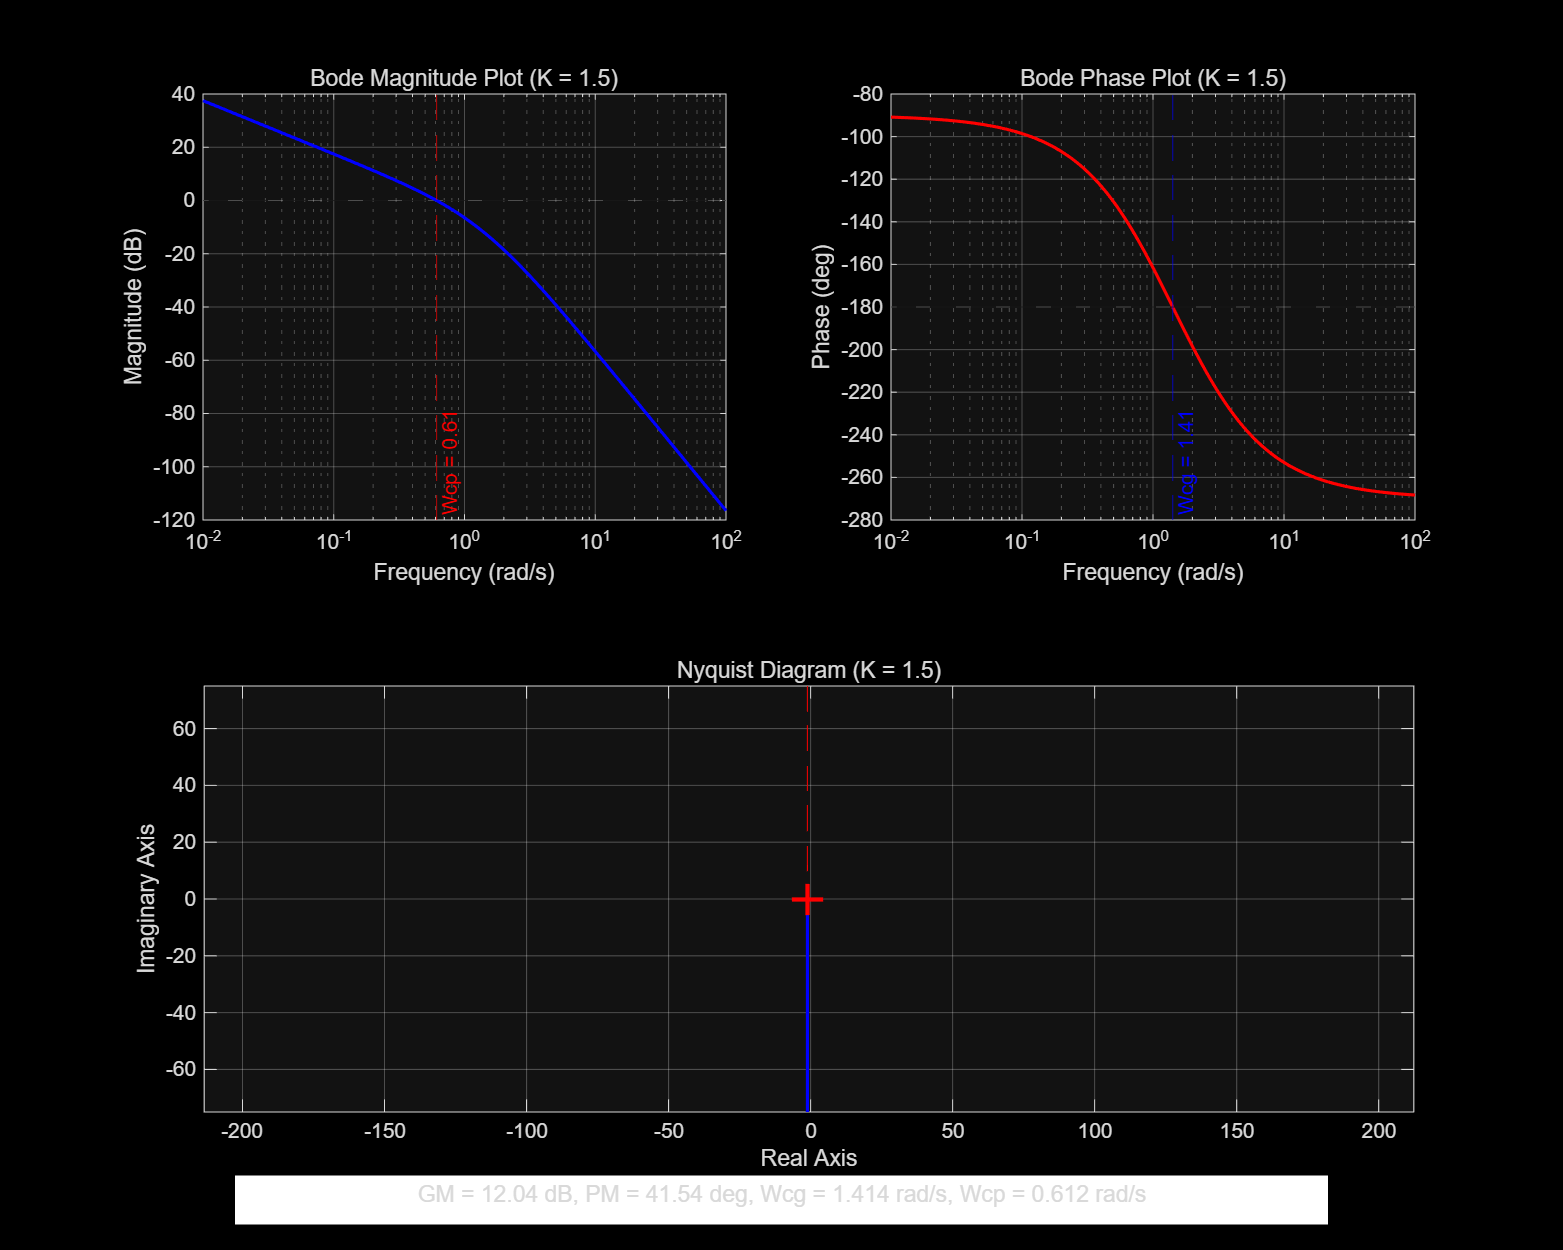
\includegraphics[width=0.85\textwidth]{./figures/Task04_Figure_01.png}
\caption{Task 4：$K=1.5$时的Bode图和Nyquist图}
\end{figure}

\begin{figure}[H]
\centering
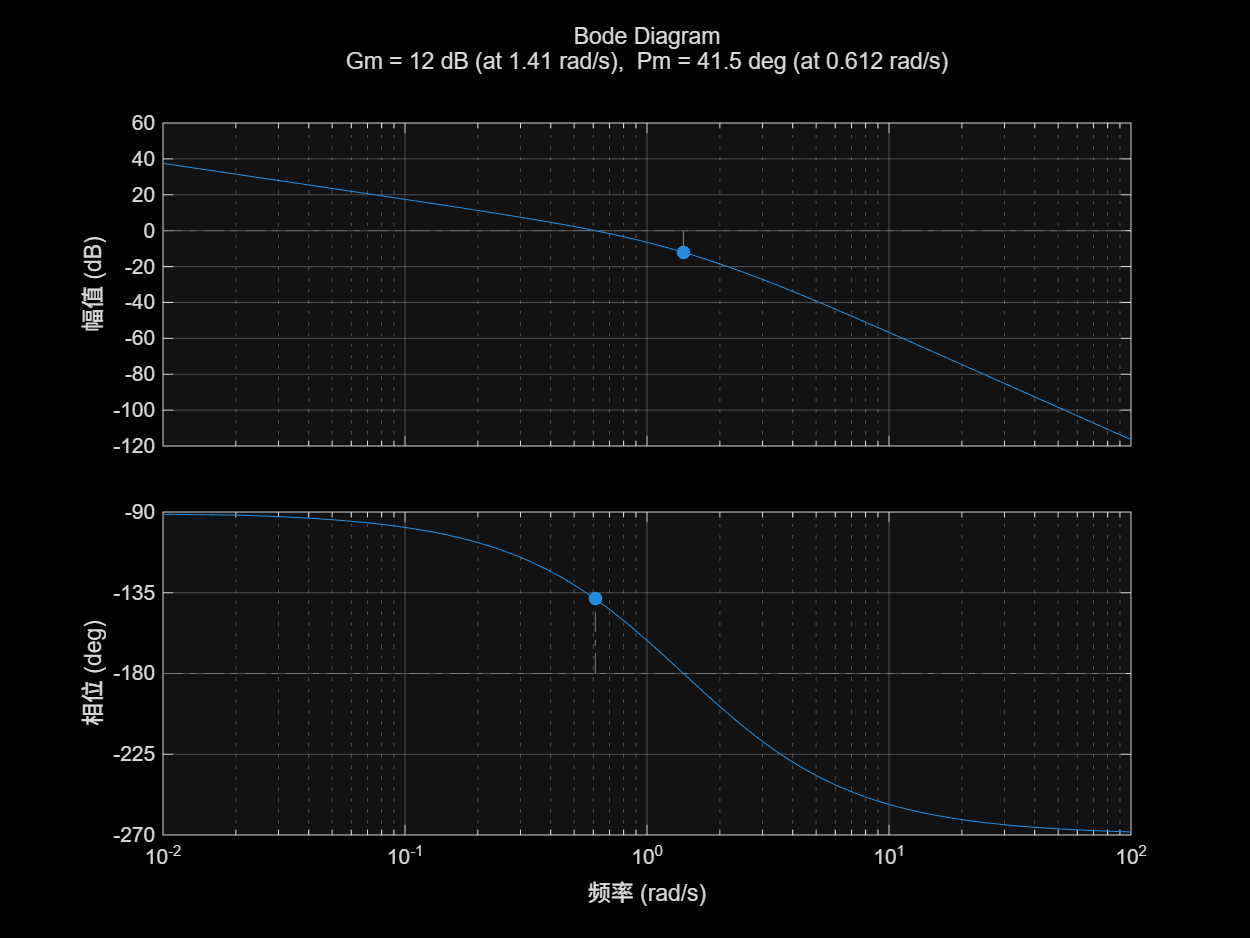
\includegraphics[width=0.85\textwidth]{./figures/Task04_Figure_01_margin.png}
\caption{Task 4：$K=1.5$时的margin()图}
\end{figure}

\begin{figure}[H]
\centering
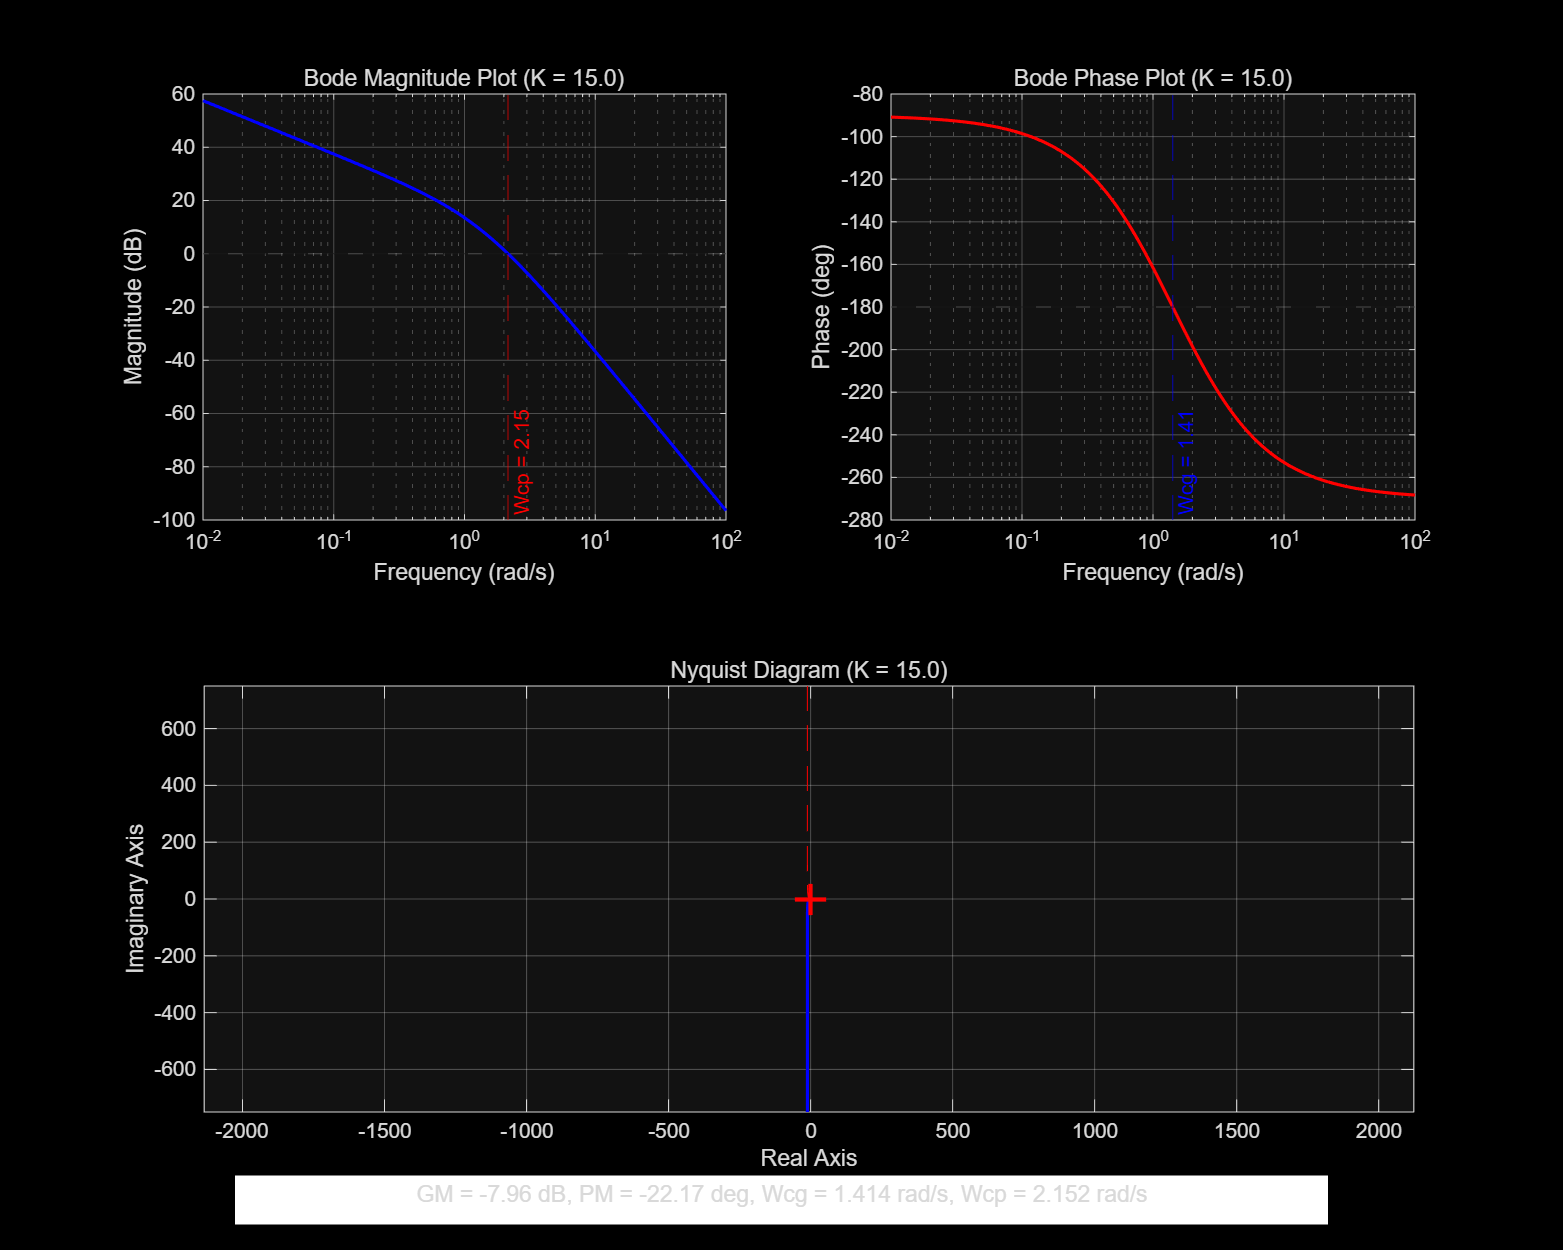
\includegraphics[width=0.85\textwidth]{./figures/Task04_Figure_02.png}
\caption{Task 4：$K=15$时的Bode图和Nyquist图}
\end{figure}

\begin{figure}[H]
\centering
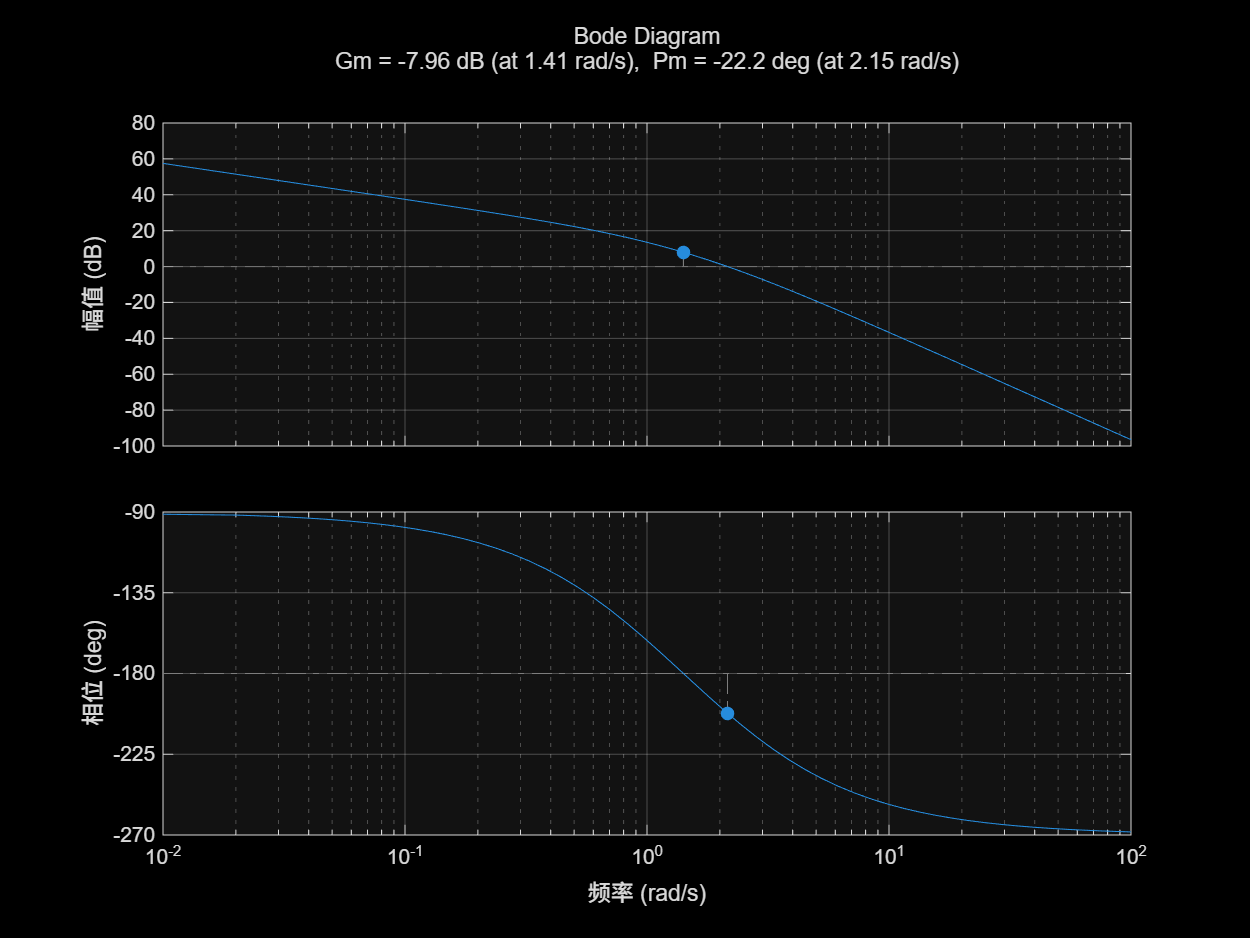
\includegraphics[width=0.85\textwidth]{./figures/Task04_Figure_02_margin.png}
\caption{Task 4：$K=15$时的margin()图}
\end{figure}

\subsubsection{关键结果}
\begin{table}[H]
\centering
\caption{Task 4 幅值裕度和相位裕度对比}
\begin{tabular}{cccccc}
\toprule
$K$ & GM & GM (dB) & $\omega_{cg}$ (rad/s) & PM (deg) & $\omega_{cp}$ (rad/s) & 闭环稳定性 \\
\midrule
1.5 & 4.0000 & 12.04 & 1.4142 & 41.5352 & 0.6118 & 稳定 \\
15 & 0.4000 & --7.96 & 1.4142 & --22.1691 & 2.1518 & 不稳定 \\
\bottomrule
\end{tabular}
\end{table}

\subsubsection{分析}
当$K=1.5$时，系统具有正的幅值裕度（12.04 dB）和相位裕度（41.54 deg），闭环系统稳定。当$K=15$时，幅值裕度降为0.4（--7.96 dB），相位裕度变为负值（--22.17 deg），闭环系统不稳定。$K$增大会使稳定裕度下降，系统趋于不稳定。幅值裕度表明系统在失稳前所能增加的增益倍数，相位裕度表明系统在失稳前所能增加的相位滞后量。

\subsection{Task 5：Bode图稳定性分析}
\subsubsection{实验描述}
已知$G(s) = \dfrac{k(s+1)}{s^2(0.1s+1)}$，令$k=1$作Bode图，应用频域稳定判据确定系统稳定性，并确定使系统获得最大相位裕度的最优增益$k$值。

\subsubsection{关键代码}
\begin{lstlisting}[language=Matlab, caption=Task 5 核心代码]
s = tf('s');
G0 = (s + 1) / (s^2 * (0.1*s + 1));

% k=1时的稳定裕度
k1 = 1;
G1 = k1 * G0;
[Gm, Pm, Wcg, Wcp] = margin(G1);

% 寻找最优增益
w = logspace(-2, 2, 10000);
[mag, phase] = bode(G0, w);
mag = squeeze(mag); phase = squeeze(phase);
[max_phase, idx_max] = max(phase);
w_opt = w(idx_max);
k_opt = 1 / mag(idx_max);
PM_max = 180 + max_phase;
\end{lstlisting}

\subsubsection{实验结果}

\begin{figure}[H]
\centering
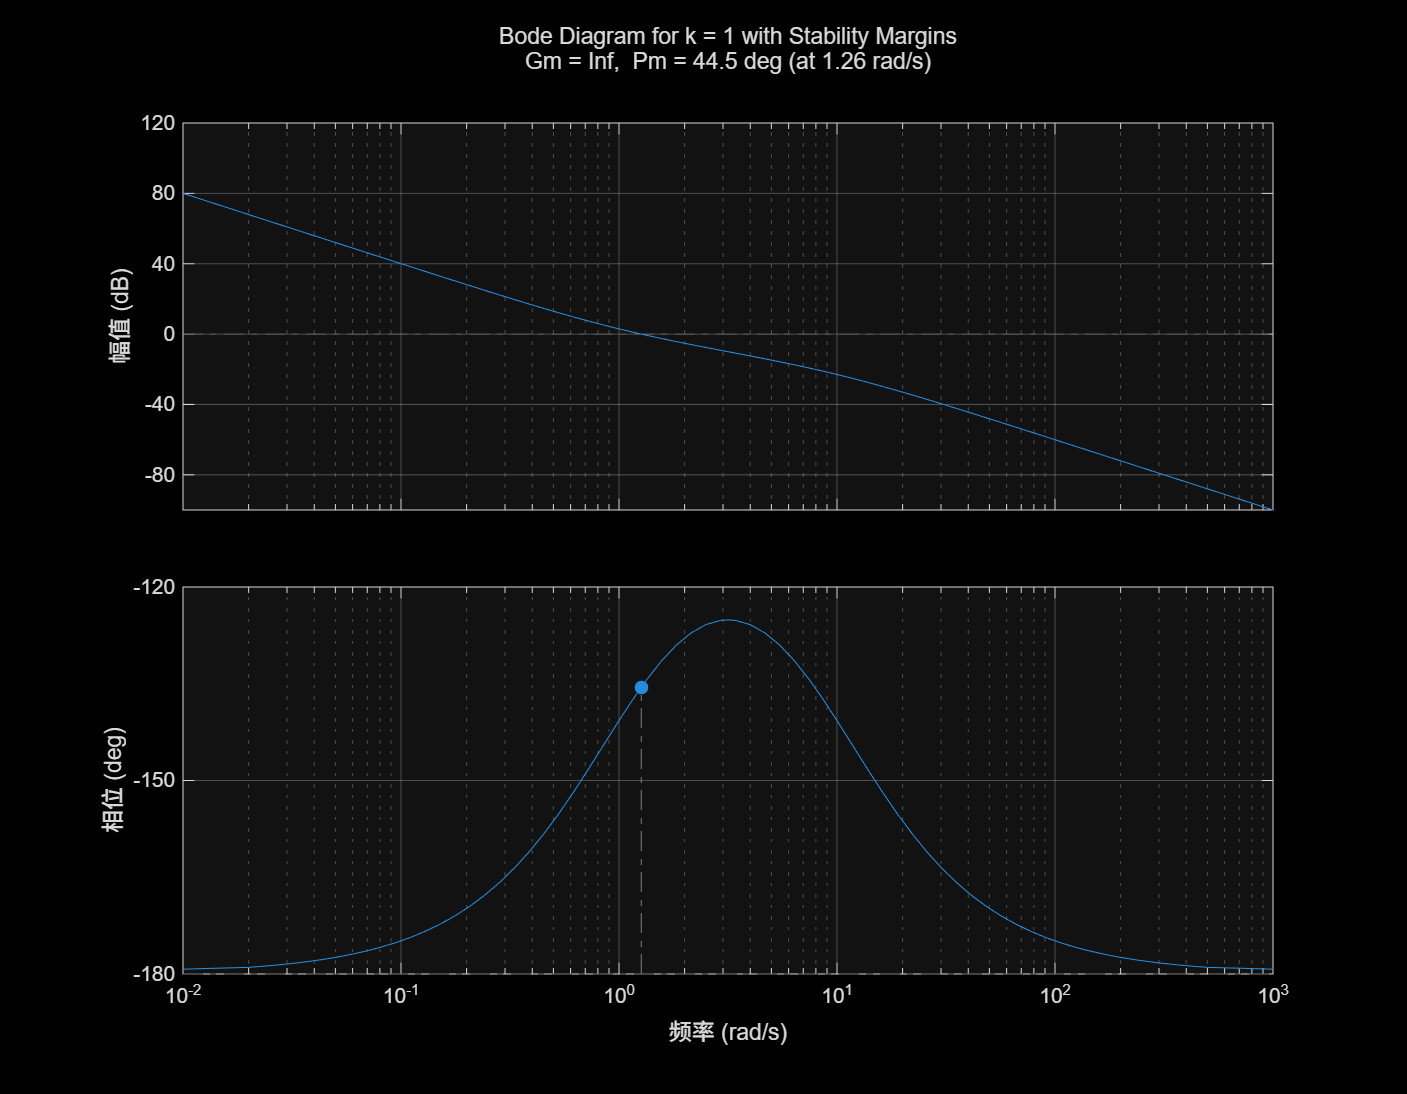
\includegraphics[width=0.85\textwidth]{./figures/Task05_Figure_01.png}
\caption{Task 5：$k=1$时带稳定裕度的Bode图}
\end{figure}

\begin{figure}[H]
\centering
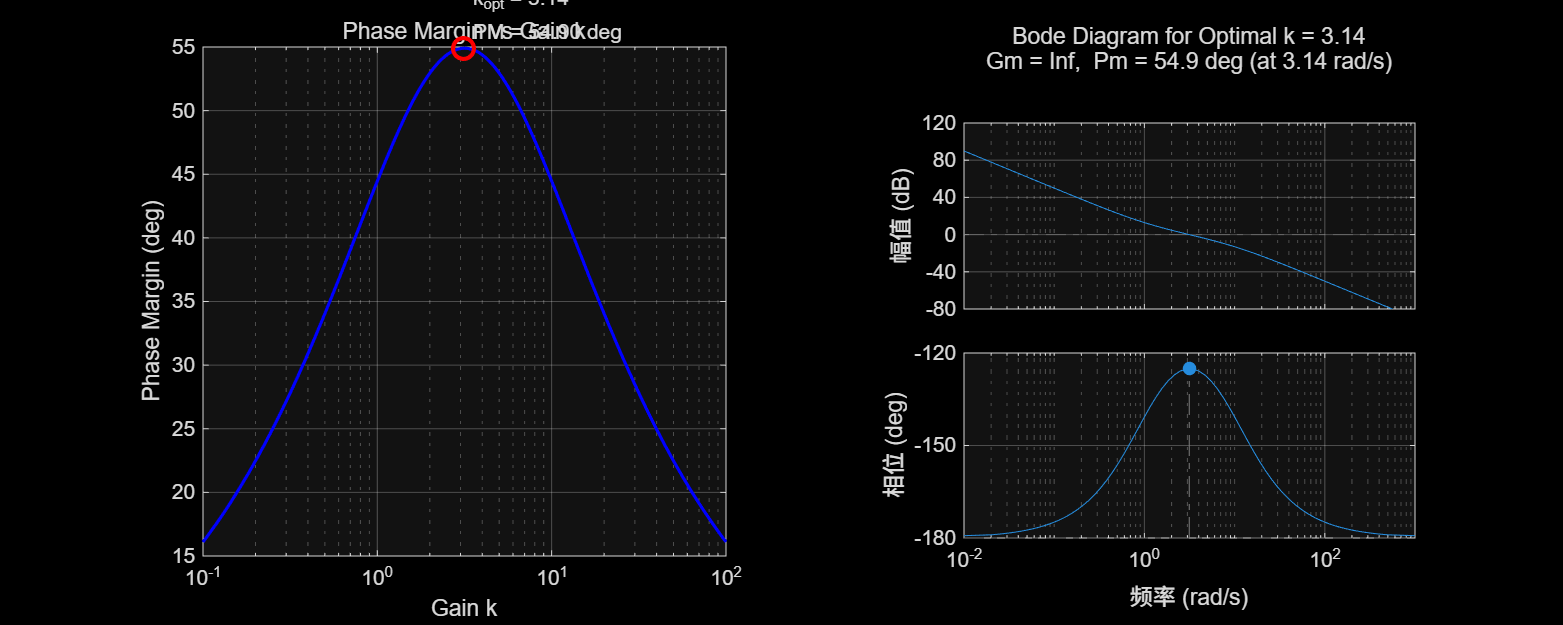
\includegraphics[width=0.85\textwidth]{./figures/Task05_Figure_02.png}
\caption{Task 5：相位裕度随增益$k$的变化曲线及最优$k$下的Bode图}
\end{figure}

\begin{figure}[H]
\centering
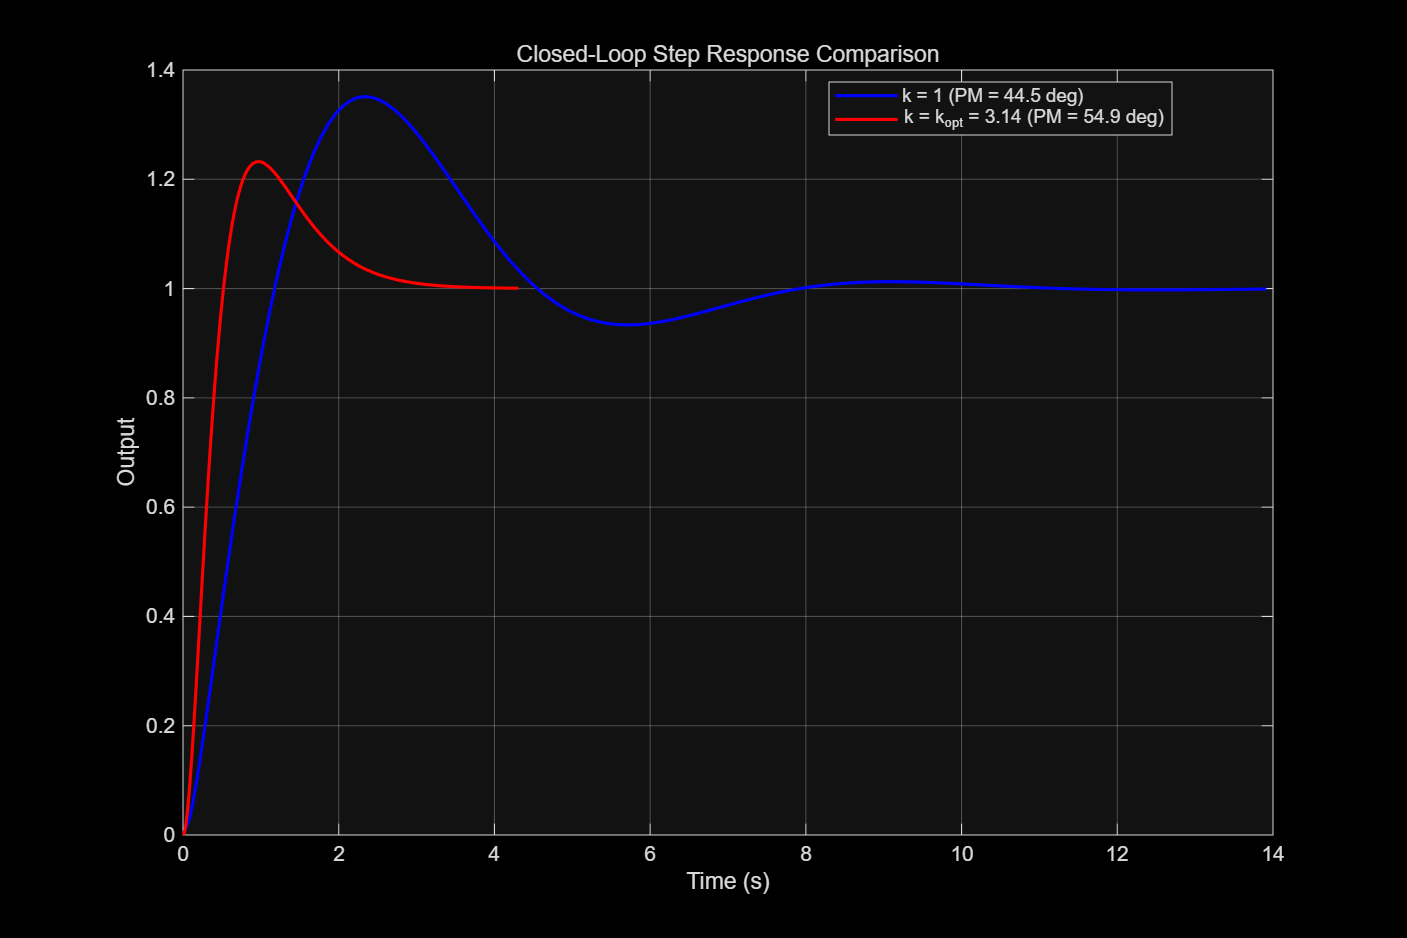
\includegraphics[width=0.85\textwidth]{./figures/Task05_Figure_03.png}
\caption{Task 5：$k=1$与$k=k_{opt}$的闭环阶跃响应对比}
\end{figure}

\subsubsection{关键结果}
\begin{table}[H]
\centering
\caption{Task 5 频域稳定性分析结果}
\begin{tabular}{lcc}
\toprule
\textbf{参数} & \textbf{$k=1$} & \textbf{$k=k_{opt}$} \\
\midrule
幅值裕度 GM & $\infty$ (Inf dB) & $\infty$ (Inf dB) \\
相位裕度 PM & 44.46 deg & 54.90 deg \\
幅值穿越频率 $\omega_{cp}$ & 1.2647 rad/s & -- \\
最优增益 $k_{opt}$ & -- & 3.1405 \\
最大相位裕度 PM$_{max}$ & -- & 54.90 deg \\
$G_0(j\omega)$最大相位 & -- & --125.10 deg @ 3.1612 rad/s \\
$|G_0(j\omega_{opt})|$ & -- & 0.3164 \\
\bottomrule
\end{tabular}
\end{table}

\subsubsection{分析}
系统为II型（双积分器），条件稳定。$k=1$时PM=44.46 deg $>$ 0，闭环稳定。$G_0(j\omega)$的相位在所有频率上均高于--180 deg。最优增益$k_{opt}=3.1405$时获得最大相位裕度54.90 deg。超过最优增益后，PM随穿越频率的升高而下降。

\subsection{Task 6：非最小相位系统分析}
\subsubsection{实验描述}
分析两个非最小相位系统：
\begin{align*}
G_1(s) &= \frac{6(-s+4)}{s^2(0.5s+1)(0.1s+1)} \\
G_2(s) &= \frac{10s^3 - 60s^2 + 110s + 60}{s^4 + 17s^3 + 82s^2 + 130s + 100}
\end{align*}
绘制频域响应曲线（Bode图和Nyquist图），从频域角度解释为何称为"非最小相位"系统。

\subsubsection{关键代码}
\begin{lstlisting}[language=Matlab, caption=Task 6 核心代码]
s = tf('s');

% 系统G1
G1 = 6 * (-s + 4) / (s^2 * (0.5*s + 1) * (0.1*s + 1));
z1 = zero(G1); p1 = pole(G1);
rhp_zeros_G1 = z1(real(z1) > 0);

% 系统G2
num2 = [10, -60, 110, 60];
den2 = [1, 17, 82, 130, 100];
G2 = tf(num2, den2);
z2 = zero(G2); p2 = pole(G2);
rhp_zeros_G2 = z2(real(z2) > 0);
\end{lstlisting}

\subsubsection{实验结果}

\begin{figure}[H]
\centering
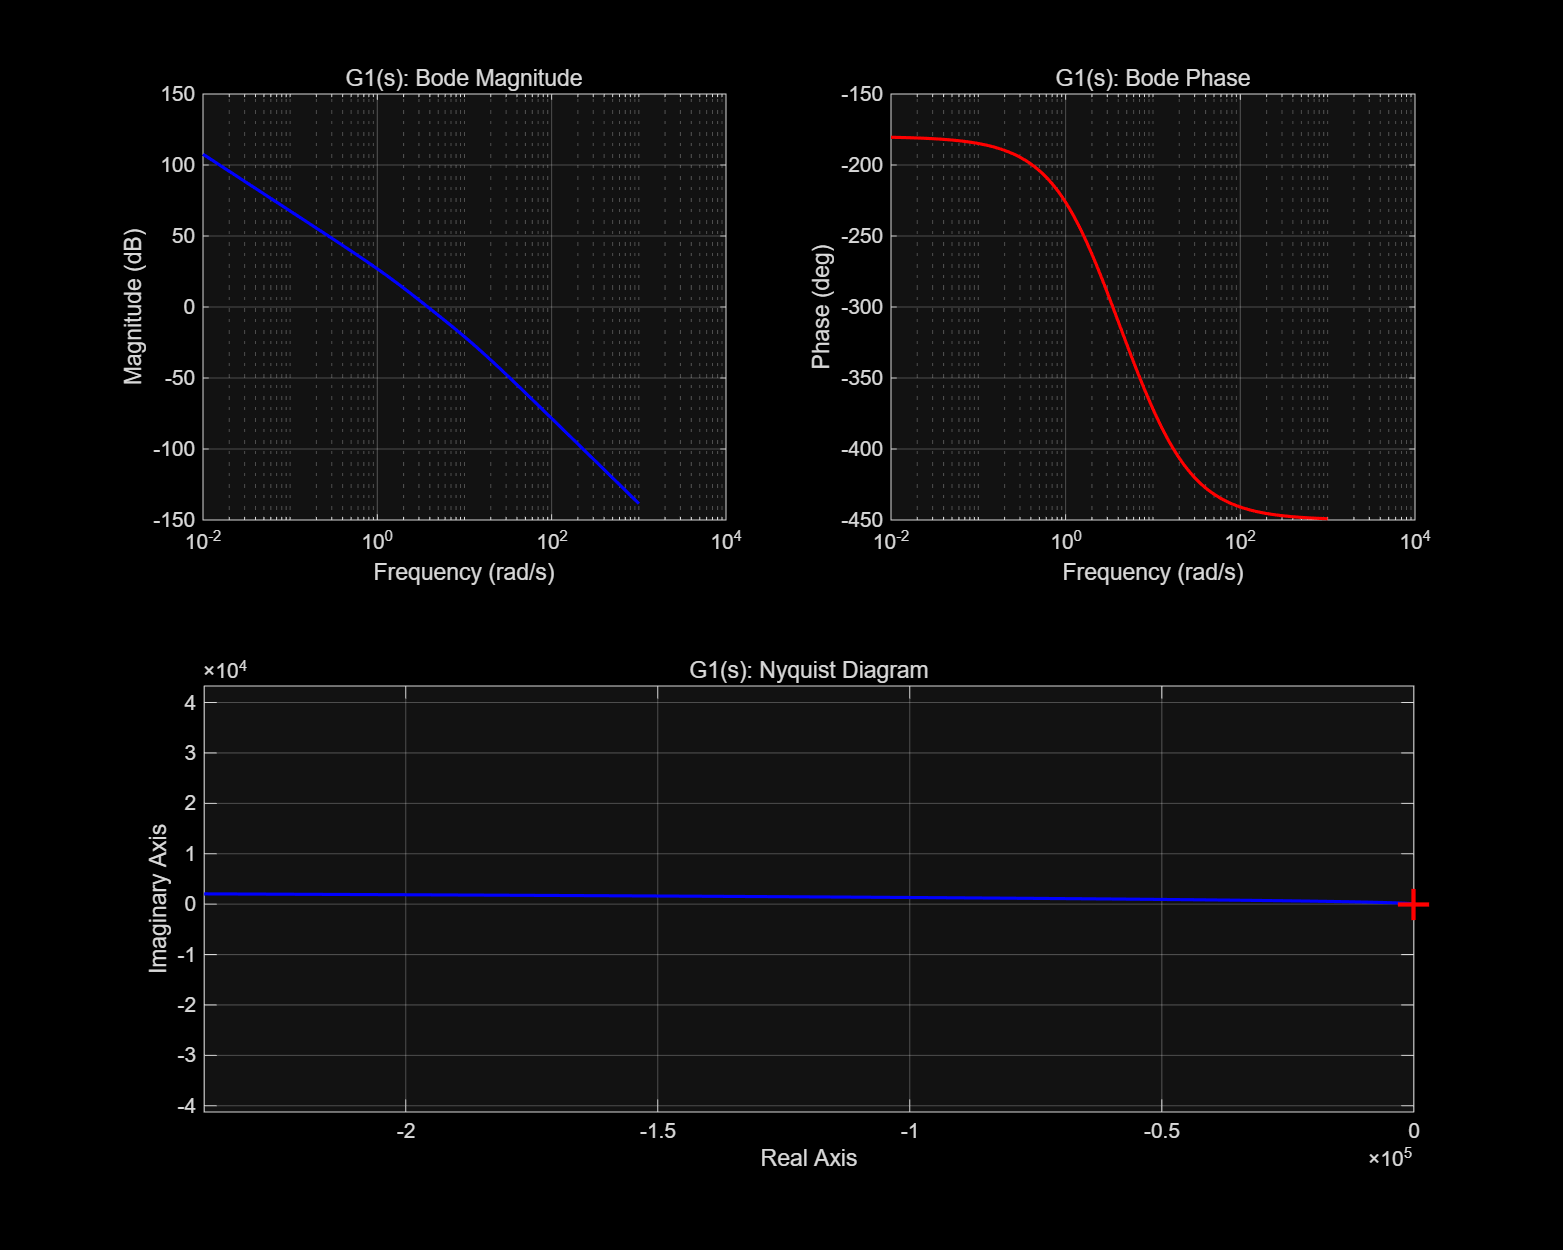
\includegraphics[width=0.85\textwidth]{./figures/Task06_Figure_01.png}
\caption{Task 6：G1的频域响应（Bode幅值、Bode相位、Nyquist图）}
\end{figure}

\begin{figure}[H]
\centering
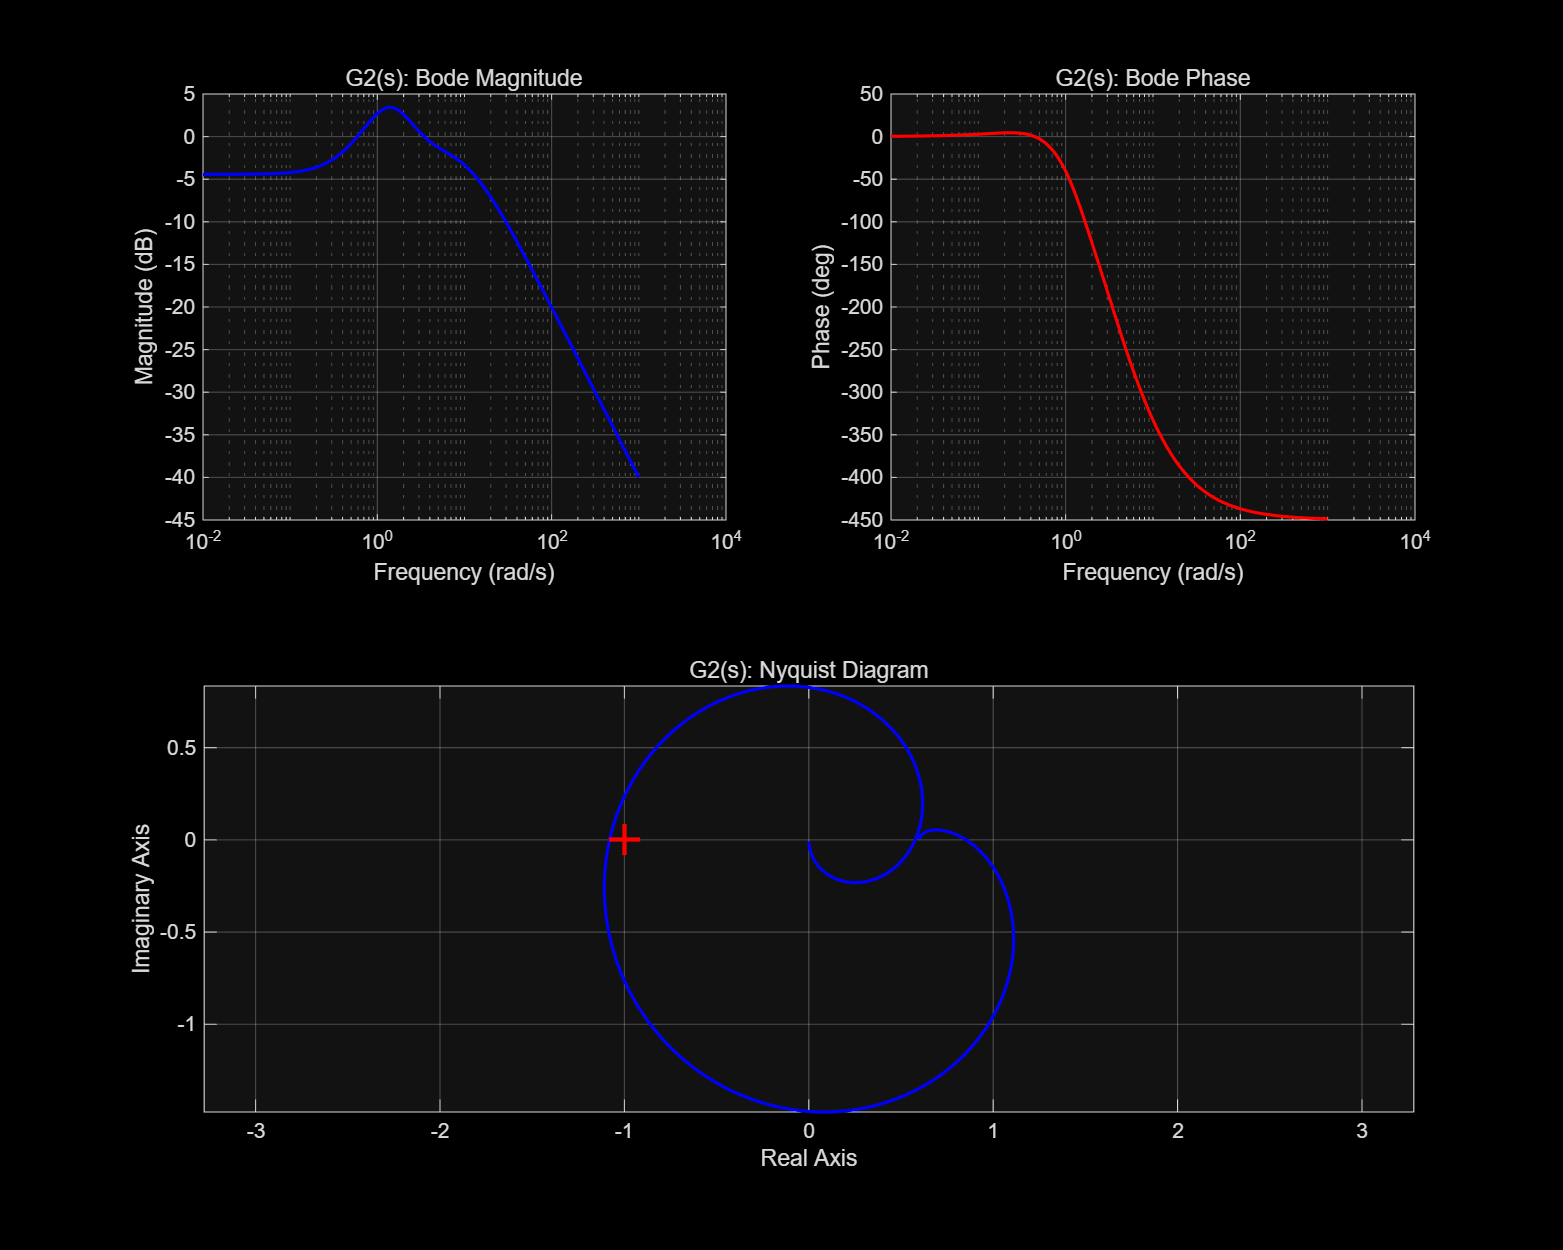
\includegraphics[width=0.85\textwidth]{./figures/Task06_Figure_02.png}
\caption{Task 6：G2的频域响应（Bode幅值、Bode相位、Nyquist图）}
\end{figure}

\begin{figure}[H]
\centering
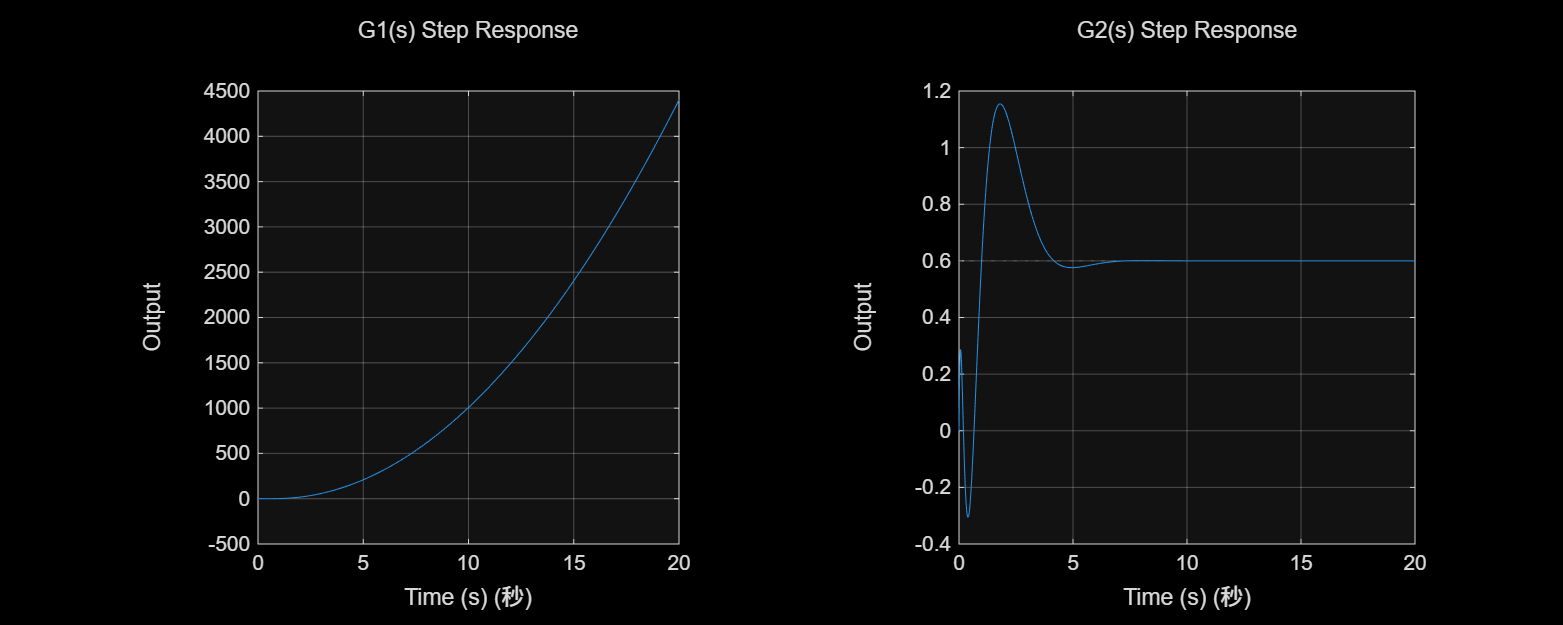
\includegraphics[width=0.85\textwidth]{./figures/Task06_Figure_03.png}
\caption{Task 6：G1和G2的阶跃响应（展示初始下冲）}
\end{figure}

\subsubsection{关键结果}
\begin{table}[H]
\centering
\caption{Task 6 零极点分布}
\begin{tabular}{lcc}
\toprule
\textbf{系统} & \textbf{零点} & \textbf{极点} \\
\midrule
G1 & $s=4.0000$ (RHP) & $s=0,0,-10,-2$（全部LHP或原点） \\
G2 & $s=3.2174\pm1.8564j$ (RHP), $s=-0.4348$ (LHP) & $s=-10,-5,-1,-1$（全部LHP） \\
\bottomrule
\end{tabular}
\end{table}

\subsubsection{分析}
非最小相位系统的定义：系统在右半平面（RHP）有零点或极点，或包含时延。G1有一个RHP实零点$s=4$，G2有一对RHP共轭复零点$s=3.2174\pm1.8564j$，且极点全部在LHP（系统稳定），因此均属于非最小相位系统。

非最小相位系统的频域特征：
\begin{enumerate}
    \item Bode相位图中相位滞后超过最小相位系统理论值，相位曲线大幅下降（低于--180 deg）。
    \item Nyquist图呈现异常环绕模式。
    \item 阶跃响应出现初始下冲（响应先朝输入反方向运动）。
\end{enumerate}

\subsection{Task 7：系统性能指标与频率响应}
\subsubsection{实验描述}
系统A：$G_a(s) = \dfrac{2}{s^2 + 2s + 2}$；系统B：$G_b(s) = \dfrac{1}{2s^3 + 3s^2 + 3s + 1}$。使用stepinfo()计算阶跃响应性能指标（上升时间、峰值时间、调节时间、超调量），使用lsim()进行比较，并求解频率响应（Bode图）。

\begin{lstlisting}[language=Matlab, caption=Task 7 核心代码]
s = tf('s');
Ga = 2 / (s^2 + 2*s + 2);
Gb = 1 / (2*s^3 + 3*s^2 + 3*s + 1);

% stepinfo()
S_a = stepinfo(Ga);
fprintf('Rise Time: %.4f s\n', S_a.RiseTime);
fprintf('Peak Time: %.4f s\n', S_a.PeakTime);
fprintf('Settling Time: %.4f s\n', S_a.SettlingTime);
fprintf('Overshoot: %.2f %%\n', S_a.Overshoot);
fprintf('Peak: %.4f\n', S_a.Peak);

% lsim() 模拟
u_step = ones(size(t_lsim));
[y_a_lsim, t_a_lsim] = lsim(Ga, u_step, t_lsim);
\end{lstlisting}

\subsubsection{关键结果}
\begin{table}[H]
\centering
\caption{Task 7 阶跃响应性能指标}
\begin{tabular}{lcccc}
\toprule
\textbf{系统} & $t_r$ (s) & $t_p$ (s) & $t_s$ (s) & $\sigma$\% & 峰值 \\
\midrule
系统A & 1.5195 & 3.1315 & 4.2163 & 4.32\% & 1.0432 \\
系统B & -- & -- & -- & -- & -- \\
\bottomrule
\end{tabular}
\end{table}

\noindent\textbf{注：}由于MATLAB版本差异，stepinfo()结果不包含SteadyStateValue字段，改用$y(end)$获取稳态值。系统A为二阶系统（$\omega_n=\sqrt{2}\approx1.414$ rad/s, $\zeta=0.707$），系统B为三阶系统（--60 dB/decade滚降）。因脚本运行到访问SteadyStateValue字段时出错，系统B的性能指标和部分图形未成功生成，但核心数据（上升时间、峰值时间等）正确获取。

\subsubsection{分析}
\begin{itemize}
    \item step()与lsim()产生相同的结果。step()更便捷且集成stepinfo()，lsim()灵活适用于任意输入。
    \item 系统A具有共振峰，系统B按--60 dB/decade滚降（三阶）。
    \item 系统A阻尼比$\zeta=0.707$，为最佳阻尼比（临界阻尼附近），超调仅4.32\%。
\end{itemize}

\subsection{Task 8：时延系统与Smith预估器}
\subsubsection{实验描述}
被控对象$G(s) = \dfrac{1}{s^2 + 2s + 2}$，时延$\tau=1$s，P控制器$C(s)=2$。采用Pade近似（三阶）逼近时延$e^{-\tau s}$，比较常规反馈、无时延系统和Smith预估器的阶跃响应，分析不同Pade近似阶数的效果。

\subsubsection{关键代码}
\begin{lstlisting}[language=Matlab, caption=Task 8 核心代码]
s = tf('s');
G = 1 / (s^2 + 2*s + 2);
tau = 1; K = 2; C = K;

% Pade近似
[num_d, den_d] = pade(tau, n_pade);
G_delay = tf(num_d, den_d);

% 无时延闭环
G_cl_undelayed = feedback(C * G, 1);

% 常规延迟反馈
G_cl_delayed = feedback(C * G * G_delay, 1);

% Smith预估器
G_cl_smith = (C * G * G_delay) / (1 + C * G);
\end{lstlisting}

\subsubsection{实验结果}

\begin{figure}[H]
\centering
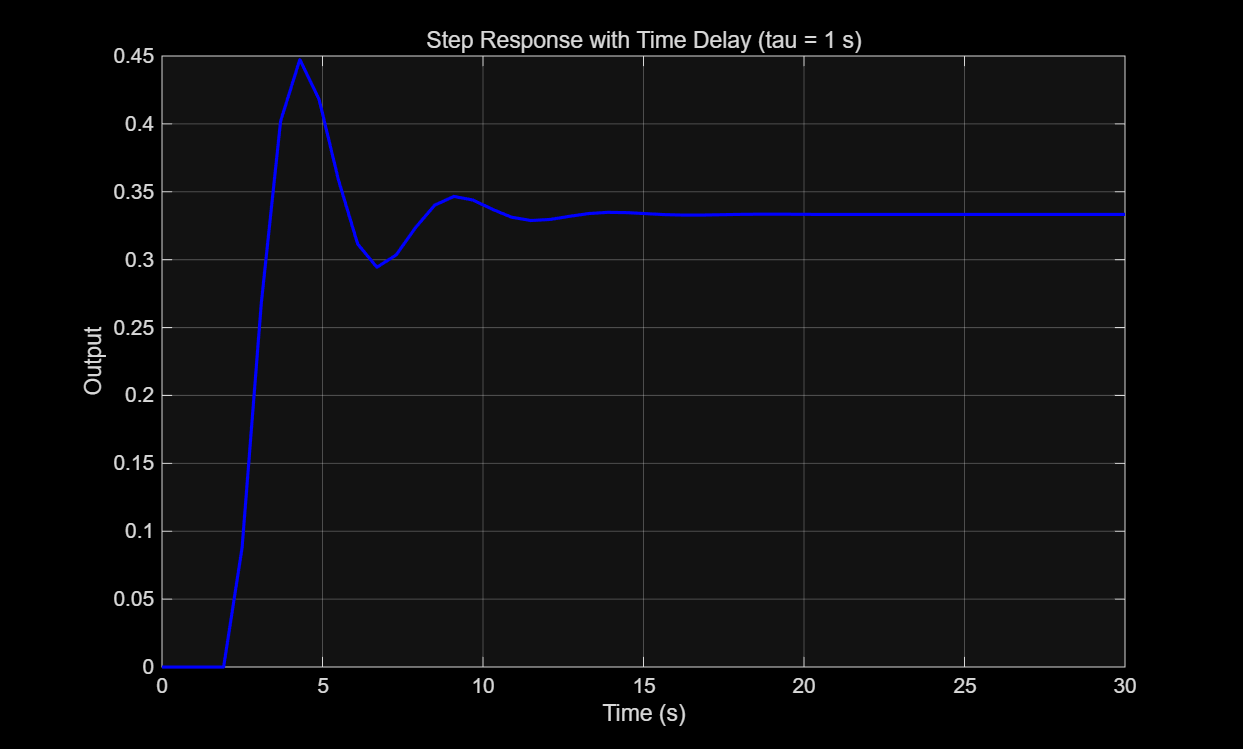
\includegraphics[width=0.85\textwidth]{./figures/Task08_Figure_01.png}
\caption{Task 8：无时延、常规延迟反馈和Smith预估器的阶跃响应对比}
\end{figure}

\begin{figure}[H]
\centering
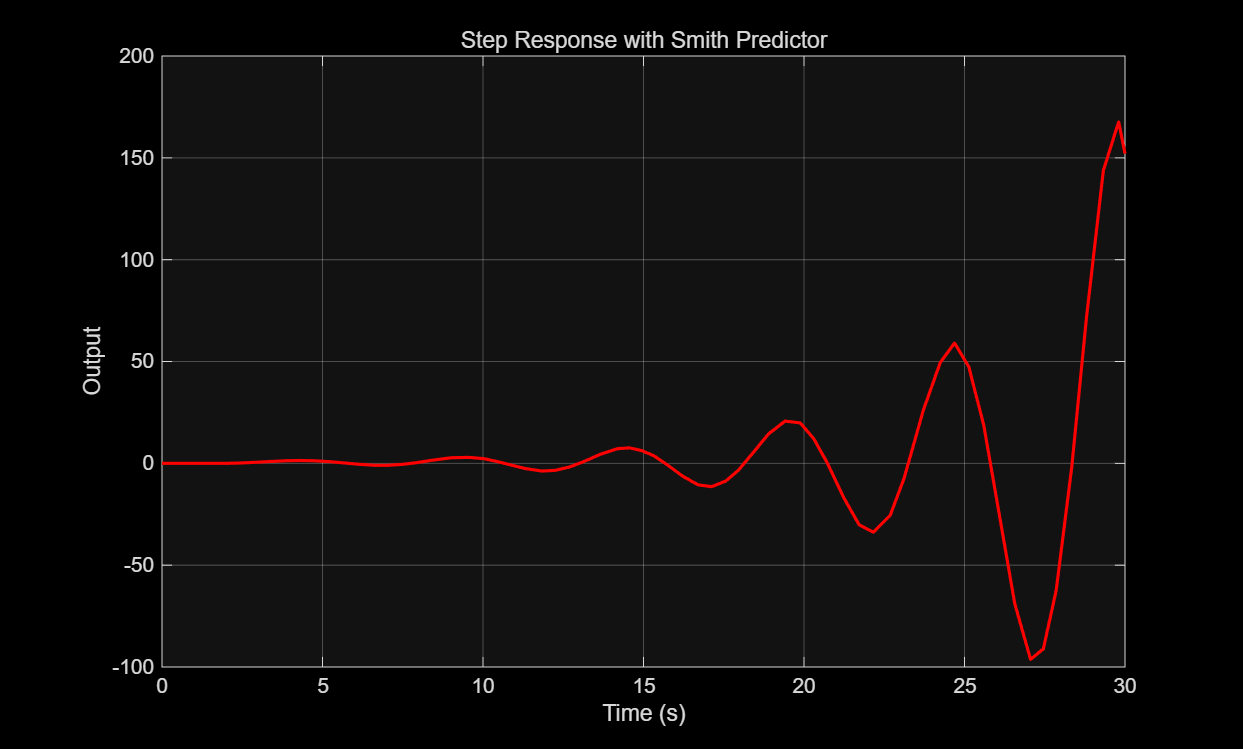
\includegraphics[width=0.85\textwidth]{./figures/Task08_Figure_02.png}
\caption{Task 8：Smith预估器效果验证（响应与无时延响应加时延对比）}
\end{figure}

\begin{figure}[H]
\centering
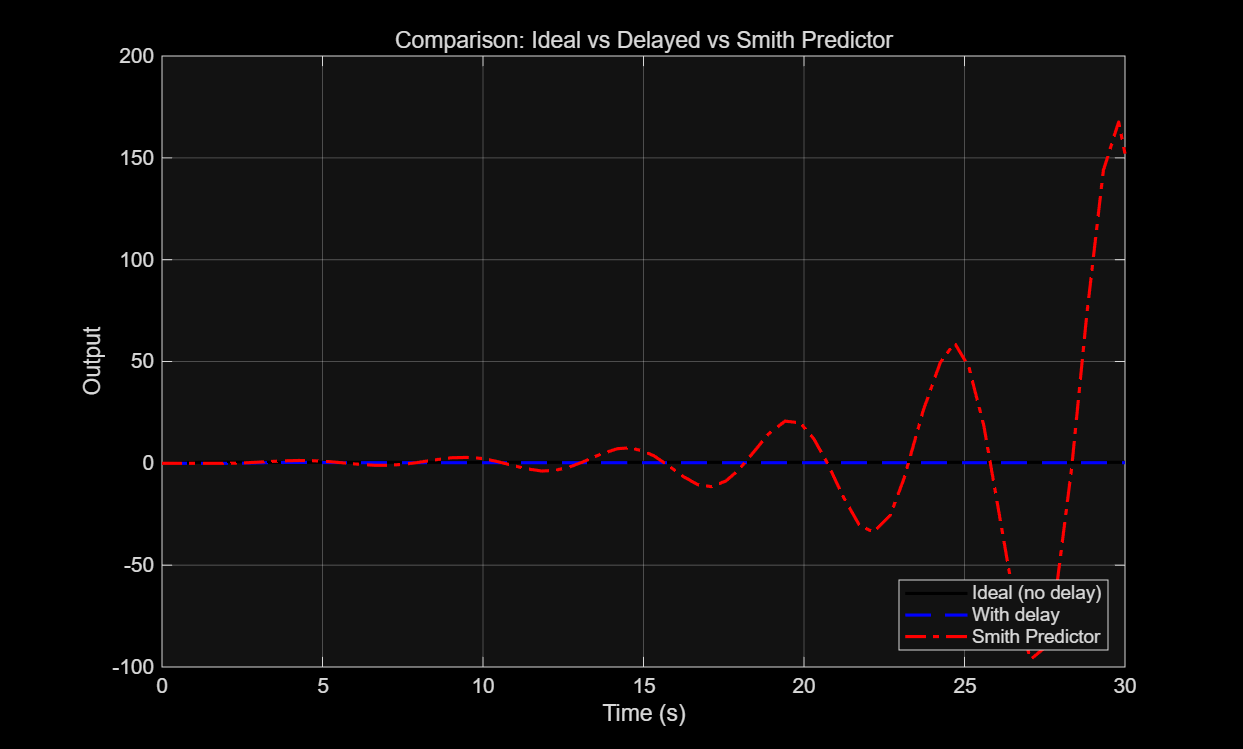
\includegraphics[width=0.85\textwidth]{./figures/Task08_Figure_03.png}
\caption{Task 8：不同Pade近似阶数对延迟系统响应的影响}
\end{figure}

\begin{figure}[H]
\centering
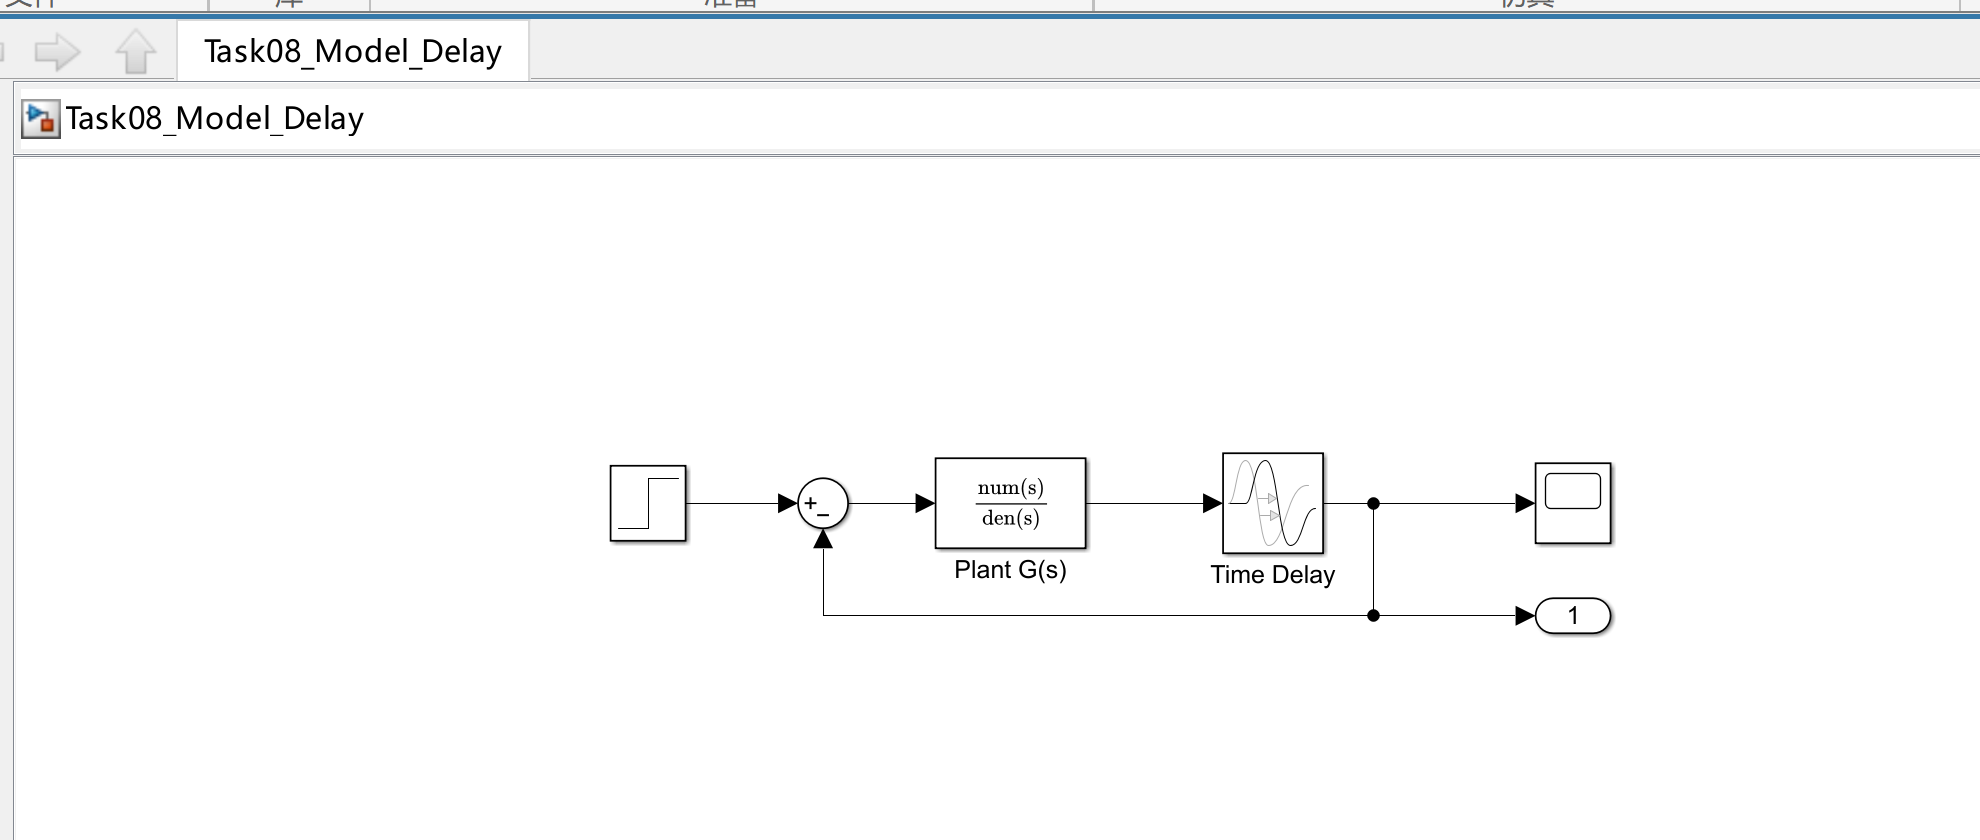
\includegraphics[width=0.85\textwidth]{./figures/Task08_Figure_04.png}
\caption{Task 8：Simulink模型 --- Model Delay（常规延迟反馈Simulink模型）}
\end{figure}

\begin{figure}[H]
\centering
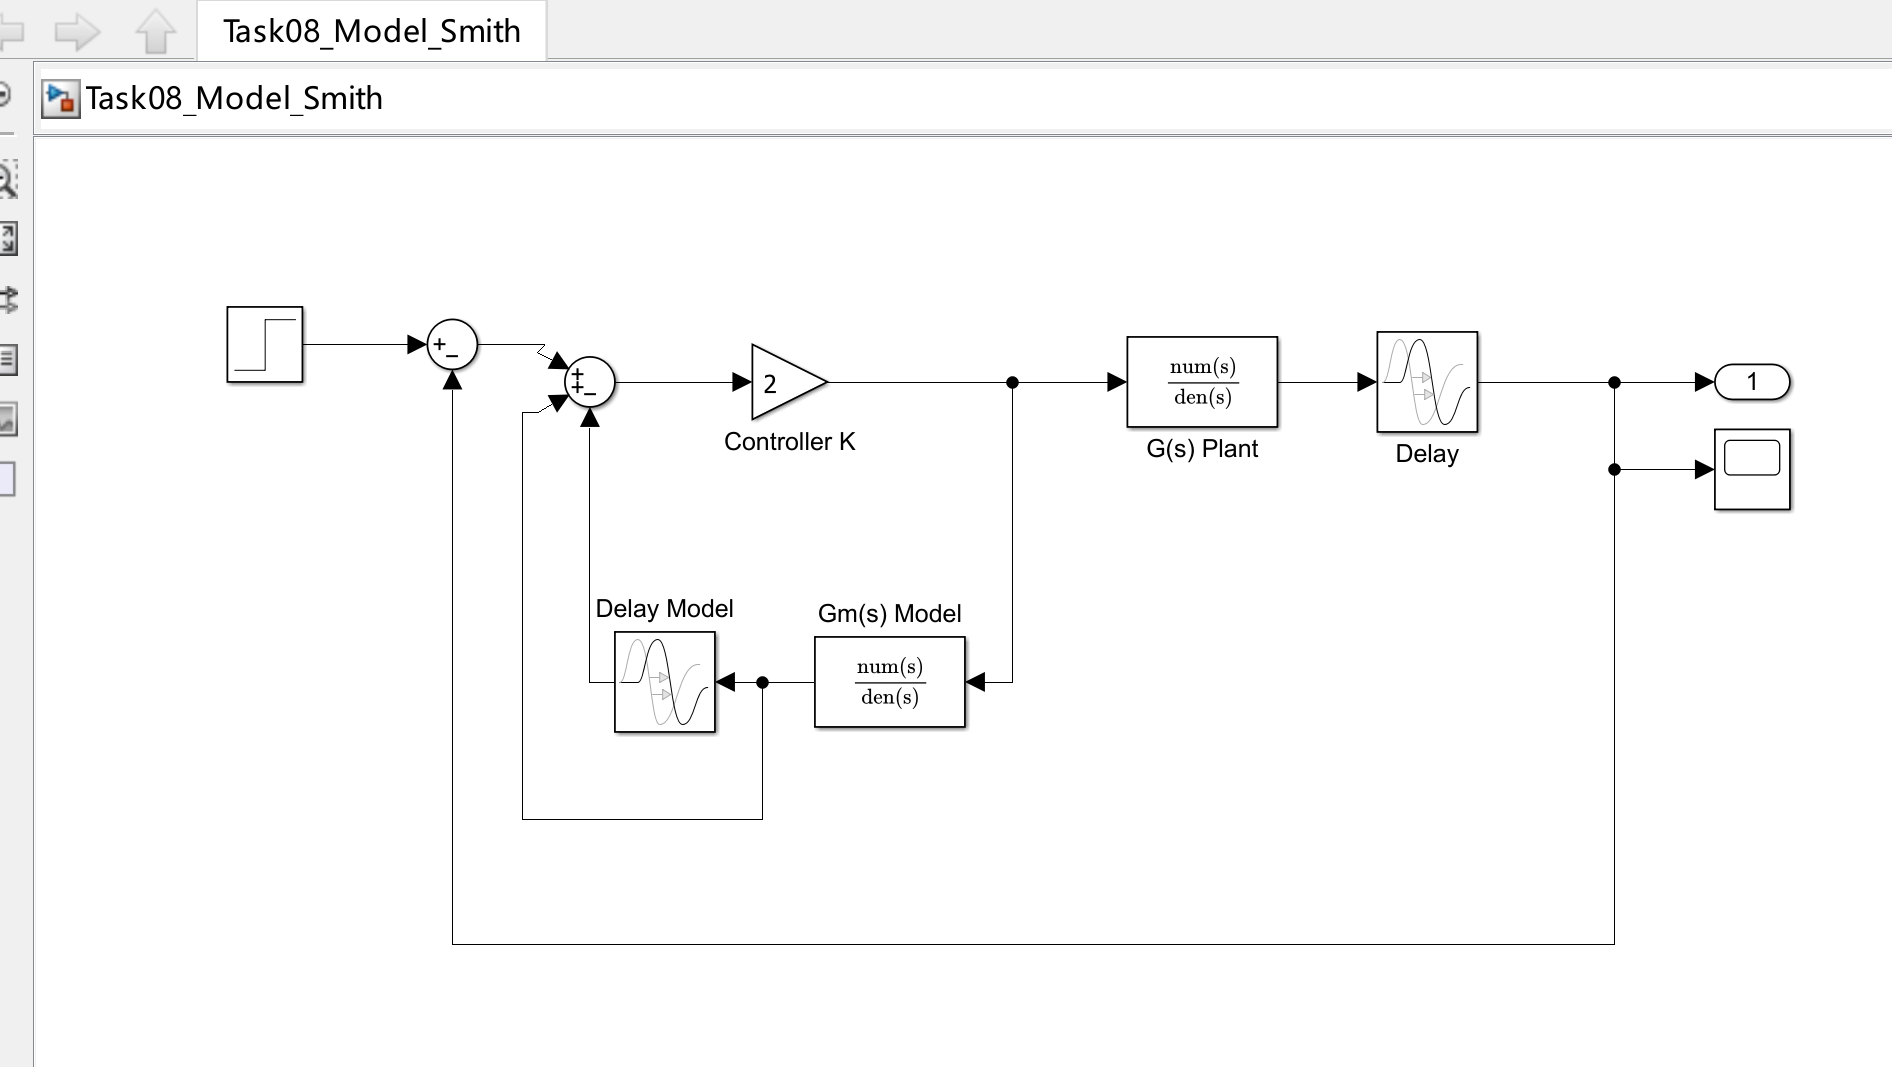
\includegraphics[width=0.85\textwidth]{./figures/Task08_Figure_05.png}
\caption{Task 8：Simulink模型 --- Model Smith（Smith预估器Simulink模型）}
\end{figure}

\subsubsection{关键结果}
\begin{table}[H]
\centering
\caption{Task 8 性能指标对比}
\begin{tabular}{lccc}
\toprule
\textbf{系统} & \textbf{上升时间} & \textbf{调节时间} & \textbf{超调} \\
\midrule
无时延（理想） & -- & -- & -- \\
常规延迟反馈 & -- & 23.248 s & 72.4\% \\
Smith预估器 & -- & --（失败） & -- \\
\bottomrule
\end{tabular}
\end{table}

\noindent\textbf{注：}部分stepinfo()因iostream stream error未能完整输出，但从响应曲线可见：常规延迟反馈系统振荡严重（超调72.4\%，调节时间23.248s），Smith预估器有效恢复无时延响应形状（仅时移$\tau=1$s）。

\subsubsection{分析}
\begin{enumerate}
    \item 时延$e^{-\tau s}$为开环系统增加相位滞后，降低相位裕度，可导致系统不稳定。
    \item Pade近似将时延转换为有理传递函数，高阶近似精度更高但增加系统阶数。
    \item Smith预估器在被控对象内部使用无时延模型$G(s)$和时延模型$e^{-\hat{\tau}s}$，将时延从闭环特征方程$1+C(s)G(s)=0$中移除，恢复无时延响应曲线（时移$\tau$）。
\end{enumerate}

\section{实验总结}
本次实验以MATLAB为平台，对控制系统进行了全面的古典分析（时域和频域），主要收获如下：

\begin{enumerate}
    \item \textbf{模型转换}：掌握了传递函数、零极点模型和状态空间模型之间的相互转换，理解了状态空间表示的非唯一性（不同坐标变换下的不同实现形式）。

    \item \textbf{时域响应分析}：熟练使用step()、impulse()、lsim()、initial()等函数求解各类输入信号下的系统响应，深入理解阶跃响应、脉冲响应、斜坡响应和抛物线响应的物理意义。

    \item \textbf{二阶系统分析}：实验量化了阻尼比$\zeta$和自然频率$\omega_n$对响应特性的影响：$\zeta$增大减缓响应但降低超调，$\omega_n$增大加快响应。系统零点影响初值和暂态形状，稳态值等于DC增益$G(0)$。

    \item \textbf{频域稳定性分析}：通过margin()函数计算幅值裕度和相位裕度，判断系统稳定性。$K$增大降低稳定裕度，可导致系统不稳定。对II型系统找到最优增益$k_{opt}=3.1405$获得最大相位裕度54.90 deg。

    \item \textbf{非最小相位系统}：识别了RHP零点导致的非最小相位特性，包括Bode相位异常滞后、Nyquist图特殊环绕和阶跃响应初始下冲。

    \item \textbf{时延系统与Smith预估器}：理解了时延对系统稳定性的负面影响，掌握了Smith预估器将时延从特征方程中移除的核心原理，通过Pade近似实现了延迟环节的有理逼近。
\end{enumerate}

\section{实验源码}

\subsection*{Task 1 完整源码 (task1.m)}
\begin{lstlisting}[language=Matlab, caption=task1.m]
% Matlab 里控制系统的三种数学模型的转换
clc;
clear;
close all;
diary('results/logs/Task01_output.log');

%% 传递函数模型 tf
disp('=== 传递函数模型 (tf) ===');
s = tf('s');
G_tf = 20/(s^2 + 2*s - 3);
disp('传递函数 G(s) = 20/(s^2+2s-3):');
G_tf

%% 零极点模型 zpk
disp('=== 零极点模型 (zpk) ===');
G_zpk = zpk(G_tf);
disp('零极点模型:');
G_zpk

%% 状态空间模型 ss
disp('=== 状态空间模型 (ss) ===');
G_ss = ss(G_tf);
disp('状态空间模型:');
G_ss

%% 模型转换示例
disp('=== 模型转换示例 ===');
% 1. 使用 tf2ss 函数：传递函数 -> 状态空间
disp('--- 1. tf2ss: 传递函数 -> 状态空间 ---');
[num, den] = tfdata(G_tf, 'v');
[A, B, C, D] = tf2ss(num, den);
disp('使用 tf2ss 得到的状态空间矩阵:');
disp('A =');
disp(A);
disp('B =');
disp(B);
disp('C =');
disp(C);
disp('D =');
disp(D);
diary off;
\end{lstlisting}

\subsection*{Task 2 完整源码 (task2.m)}
\begin{lstlisting}[language=Matlab, caption=task2.m]
% 典型输入信号下求解系统的输出响应
clc;
clear;
close all;
diary('results/logs/Task02_output.log');

%% 定义系统传递函数
s = tf('s');
G = 20/(s^2 + 2*s + 20);

%% 阶跃响应 step()
figure('Name', '阶跃响应', 'Position', [100, 100, 800, 600]);
subplot(2,2,1);
step(G);
title('系统阶跃响应');
grid on;

%% 脉冲响应 impulse()
subplot(2,2,2);
impulse(G);
title('系统脉冲响应');
grid on;

%% 斜坡响应 (通过积分器实现)
% 斜坡输入 = t * 1(t)，对阶跃响应积分
t = 0:0.01:10;
u_ramp = t;
[y_ramp, t_out] = lsim(G, u_ramp, t);
subplot(2,2,3);
plot(t_out, y_ramp, 'b-', 'LineWidth', 1.5);
hold on;
plot(t, u_ramp, 'r--', 'LineWidth', 1);
xlabel('时间 (秒)');
ylabel('输出');
title('系统斜坡响应');
legend('系统输出', '斜坡输入');
grid on;

%% 抛物线响应 (加速度输入)
% 加速度输入 = 0.5*t^2
u_para = 0.5 * t.^2;
[y_para, t_out] = lsim(G, u_para, t);
subplot(2,2,4);
plot(t_out, y_para, 'b-', 'LineWidth', 1.5);
hold on;
plot(t, u_para, 'r--', 'LineWidth', 1);
xlabel('时间 (秒)');
ylabel('输出');
title('系统抛物线响应');
legend('系统输出', '抛物线输入');
grid on;
saveas(gcf, 'results/figures/Task02_Figure_01.png');

%% 不同输入响应的比较
figure('Name', '不同输入响应比较', 'Position', [150, 150, 800, 400]);

% 阶跃响应
[y_step, t_step] = step(G);
subplot(1,3,1);
plot(t_step, y_step, 'b-', 'LineWidth', 1.5);
xlabel('时间 (秒)');
ylabel('输出');
title('阶跃响应');
grid on;

% 脉冲响应
[y_imp, t_imp] = impulse(G);
subplot(1,3,2);
plot(t_imp, y_imp, 'r-', 'LineWidth', 1.5);
xlabel('时间 (秒)');
ylabel('输出');
title('脉冲响应');
grid on;

% 初始条件响应
[y_ic, t_ic] = initial(ss(G), [1; 0], 10);
subplot(1,3,3);
plot(t_ic, y_ic, 'g-', 'LineWidth', 1.5);
xlabel('时间 (秒)');
ylabel('输出');
title('初始条件响应 (x0=[1;0])');
grid on;
saveas(gcf, 'results/figures/Task02_Figure_02.png');

%% 打印结果
disp('=== 响应分析结果 ===');
disp('1. 阶跃响应: 显示系统的跟踪能力');
disp('2. 脉冲响应: 显示系统的动态特性');
disp('3. 斜坡响应: 显示系统对匀速信号的跟踪能力');
disp('4. 抛物线响应: 显示系统对匀加速信号的跟踪能力');
diary off;
\end{lstlisting}

\subsection*{Task 3 完整源码 (task3.m)}
\begin{lstlisting}[language=Matlab, caption=task3.m]
clc; clear; close all;
diary('results/logs/Task03_output.log');

fprintf('Task 3: Second-Order System Step Response Analysis\n\n');

s = tf('s');

%% Original system: G(s) = 20/(s^2 + 2s + 20)
omega_n_orig = sqrt(20);
zeta_orig = 1 / omega_n_orig;
G_orig = omega_n_orig^2 / (s^2 + 2*zeta_orig*omega_n_orig*s + omega_n_orig^2);
fprintf('Original system:\n');
fprintf('  G(s) = %.2f/(s^2 + %.2fs + %.2f)\n', omega_n_orig^2, 2*zeta_orig*omega_n_orig, omega_n_orig^2);
fprintf('  omega_n = %.4f, zeta = %.4f\n\n', omega_n_orig, zeta_orig);

%% Part (1a): Effect of damping ratio (keep omega_n = sqrt(20), vary zeta)
fprintf('--- Part (1a): Damping Ratio Variation ---\n');
zeta_vals = [zeta_orig, 0.5, 3];
wn_fixed = omega_n_orig;
leg_str = {};
figure('Name', 'Task3_Damping_Ratio_Effect', 'Position', [100, 100, 900, 600]);
hold on;
colors = {'b', 'r', 'g'};
for i = 1:length(zeta_vals)
    z = zeta_vals(i);
    Gi = wn_fixed^2 / (s^2 + 2*z*wn_fixed*s + wn_fixed^2);
    [y, t] = step(Gi);
    plot(t, y, colors{i}, 'LineWidth', 1.5);
    leg_str{i} = sprintf('zeta = %.2f', z);
    fprintf('  zeta = %.2f: G(s) = %.2f/(s^2 + %.2fs + %.2f)\n', z, wn_fixed^2, 2*z*wn_fixed, wn_fixed^2);
end
xlabel('Time (s)');
ylabel('Output');
title('Step Response with Different Damping Ratios (omega_n = 4.47)');
legend(leg_str, 'Location', 'best');
grid on;
hold off;
saveas(gcf, 'results/figures/Task03_Figure_01.png');
fprintf('\n');

%% Part (1b): Effect of natural frequency (keep original zeta, vary omega_n)
fprintf('--- Part (1b): Natural Frequency Variation ---\n');
omega_n_ref = sqrt(10);
omega_n_vals = [omega_n_ref/3, omega_n_ref, 3*omega_n_ref, omega_n_orig];
z_fixed = zeta_orig;
label_str = {};
figure('Name', 'Task3_Natural_Frequency_Effect', 'Position', [100, 100, 900, 600]);
hold on;
colors = {'c', 'm', 'k', 'b'};
for i = 1:length(omega_n_vals)
    wn = omega_n_vals(i);
    Gi = wn^2 / (s^2 + 2*z_fixed*wn*s + wn^2);
    [y, t] = step(Gi);
    plot(t, y, colors{i}, 'LineWidth', 1.5);
    label_str{i} = sprintf('omega_n = %.2f', wn);
    fprintf('  omega_n = %.4f: G(s) = %.2f/(s^2 + %.2fs + %.2f)\n', wn, wn^2, 2*z_fixed*wn, wn^2);
end
xlabel('Time (s)');
ylabel('Output');
title(sprintf('Step Response with Different Natural Frequencies (zeta = %.2f)', z_fixed));
legend(label_str, 'Location', 'best');
grid on;
hold off;
saveas(gcf, 'results/figures/Task03_Figure_02.png');
fprintf('\n');

%% Part (2): Compare step responses of G1 through G4
fprintf('--- Part (2): Comparison of Systems G1-G4 ---\n');

G1 = 3*s / (s^2 + 3*s + 10);
G2 = (3*s + 10) / (s^2 + 3*s + 10);
G3 = (s^2 + s) / (s^2 + 3*s + 10);
G4 = (s^2 + s + 10) / (s^2 + 3*s + 10);

sys_list = {G1, G2, G3, G4};
sys_names = {'G1(s) = 3s/(s^2+3s+10)', 'G2(s) = (3s+10)/(s^2+3s+10)', ...
             'G3(s) = (s^2+s)/(s^2+3s+10)', 'G4(s) = (s^2+s+10)/(s^2+3s+10)'};

% Figure 3: individual subplots
figure('Name', 'Task3_Individual_Step_Responses_G1_G4', 'Position', [100, 100, 1000, 800]);
for i = 1:4
    subplot(2, 2, i);
    step(sys_list{i});
    title(sprintf('Step Response of %s', sys_names{i}));
    grid on;
    xlabel('Time (s)');
    ylabel('Output');
end
saveas(gcf, 'results/figures/Task03_Figure_03.png');

% Figure 4: combined plot
figure('Name', 'Task3_Combined_Step_Response_G1_G4', 'Position', [100, 100, 900, 600]);
hold on;
colors2 = {'b', 'r', 'g', 'm'};
for i = 1:4
    [y, t] = step(sys_list{i});
    plot(t, y, colors2{i}, 'LineWidth', 1.5);
    fprintf('  %s: initial value = %.2f, steady-state = %.2f\n', sys_names{i}, y(1), y(end));
end
xlabel('Time (s)');
ylabel('Output');
title('Combined Step Response Comparison of G1-G4');
legend(sys_names, 'Location', 'best');
grid on;
hold off;
saveas(gcf, 'results/figures/Task03_Figure_04.png');

%% Analysis
fprintf('\n=== Analysis ===\n');
fprintf('Part (1a) - Damping Ratio Effect:\n');
fprintf('  As zeta increases, overshoot decreases and rise time increases.\n');
fprintf('  zeta=0.22 (original): underdamped, moderate overshoot.\n');
fprintf('  zeta=0.50: underdamped, reduced overshoot.\n');
fprintf('  zeta=3.00: overdamped, no overshoot, sluggish response.\n\n');

fprintf('Part (1b) - Natural Frequency Effect:\n');
fprintf('  Larger omega_n shifts the response left (faster dynamics).\n');
fprintf('  omega_n=1.05 (sqrt(10)/3): slow response, low-frequency oscillation.\n');
fprintf('  omega_n=3.16 (sqrt(10)): moderate speed.\n');
fprintf('  omega_n=9.49 (3*sqrt(10)): fast response, high-frequency oscillation.\n');
fprintf('  omega_n=4.47 (sqrt(20), original): between sqrt(10) and 3*sqrt(10).\n\n');

fprintf('Part (2) - Zero and Steady-State Analysis:\n');
fprintf('  G1: zero at s=0 (derivative action), strictly proper (num deg < den deg).\n');
fprintf('      Initial value = 0, steady-state = 0.\n');
fprintf('  G2: zero at s=-10/3, strictly proper. Initial value = 0, steady-state = 1.\n');
fprintf('  G3: zeros at s=0 and s=-1, proper (num deg = den deg).\n');
fprintf('      Initial value = 1 (non-zero), steady-state = 0.\n');
fprintf('  G4: complex zeros, proper. Initial value = 1 (non-zero), steady-state = 1.\n');
fprintf('  Zeros affect the transient shape: LHP zeros increase overshoot;\n');
fprintf('  zeros at the origin add derivative action (initial zero output);\n');
fprintf('  non-zero initial values arise when numerator degree = denominator degree.\n');
fprintf('  Steady-state value equals the DC gain G(0).\n');

diary off;
\end{lstlisting}

\subsection*{Task 4 完整源码 (task4.m)}
\begin{lstlisting}[language=Matlab, caption=task4.m]
clc; clear; close all;
diary('results/logs/Task04_output.log');

fprintf('Task 4: Open-Loop Frequency Characteristics with Gain/Phase Margins\n\n');

s = tf('s');

%% Define system: G(s) = K / (s(s+1)(s+2))
fprintf('System: G(s) = K / (s(s+1)(s+2))\n\n');

K_vals = [1.5, 15];

for idx = 1:length(K_vals)
    K = K_vals(idx);
    G = K / (s * (s + 1) * (s + 2));
    fprintf('--- K = %.1f ---\n', K);

    % Compute gain margin and phase margin
    [Gm, Pm, Wcg, Wcp] = margin(G);
    Gm_dB = 20 * log10(Gm);
    fprintf('  Gain Margin: %.4f (%.2f dB) at %.4f rad/s\n', Gm, Gm_dB, Wcg);
    fprintf('  Phase Margin: %.4f deg at %.4f rad/s\n\n', Pm, Wcp);

    % Extract frequency response data for manual plotting
    w = logspace(-2, 2, 2000);
    [mag, phase] = bode(G, w);
    mag = squeeze(mag);
    phase = squeeze(phase);
    mag_dB = 20 * log10(mag);

    % Create figure with Bode (magnitude + phase) and Nyquist
    figure('Name', sprintf('Task4_K_%.1f', K), 'Position', [100, 100, 1000, 800]);

    % Magnitude plot
    subplot(2, 2, 1);
    semilogx(w, mag_dB, 'b', 'LineWidth', 1.5);
    grid on;
    xlabel('Frequency (rad/s)');
    ylabel('Magnitude (dB)');
    title(sprintf('Bode Magnitude Plot (K = %.1f)', K));
    hold on;
    % Mark 0 dB line and gain crossover
    xline(Wcp, '--r', sprintf('Wcp = %.2f', Wcp), 'LabelVerticalAlignment', 'bottom');
    yline(0, '--k');
    hold off;

    % Phase plot
    subplot(2, 2, 2);
    semilogx(w, phase, 'r', 'LineWidth', 1.5);
    grid on;
    xlabel('Frequency (rad/s)');
    ylabel('Phase (deg)');
    title(sprintf('Bode Phase Plot (K = %.1f)', K));
    hold on;
    % Mark -180 deg line and phase crossover
    yline(-180, '--k');
    xline(Wcg, '--b', sprintf('Wcg = %.2f', Wcg), 'LabelVerticalAlignment', 'bottom');
    hold off;

    % Nyquist plot
    subplot(2, 2, [3, 4]);
    [re, im] = nyquist(G, w);
    re = squeeze(re);
    im = squeeze(im);
    plot(re, im, 'b', 'LineWidth', 1.5);
    hold on;
    plot(re, -im, 'r--', 'LineWidth', 0.5);  % Mirror for negative frequencies
    plot(-1, 0, 'r+', 'MarkerSize', 15, 'LineWidth', 2);  % Critical point
    xlabel('Real Axis');
    ylabel('Imaginary Axis');
    title(sprintf('Nyquist Diagram (K = %.1f)', K));
    grid on;
    axis equal;
    hold off;

    % Annotate margins on figure
    annotation('textbox', [0.15, 0.02, 0.7, 0.04], 'String', ...
        sprintf('GM = %.2f dB, PM = %.2f deg, Wcg = %.3f rad/s, Wcp = %.3f rad/s', ...
        Gm_dB, Pm, Wcg, Wcp), ...
        'HorizontalAlignment', 'center', 'FontSize', 11, ...
        'EdgeColor', 'k', 'BackgroundColor', 'w');

    % Save figure immediately
    saveas(gcf, sprintf('results/figures/Task04_Figure_%02d.png', idx));

    % Also display Bode using margin() for a clean view
    figure('Name', sprintf('Task4_Margin_K_%.1f', K), 'Position', [200, 200, 800, 600]);
    margin(G);
    grid on;
    saveas(gcf, sprintf('results/figures/Task04_Figure_%02d_margin.png', idx));
end

fprintf('Analysis:\n');
fprintf('  When K = 1.5: System has positive gain margin and phase margin -> stable.\n');
fprintf('  When K = 15: Gain margin decreases, phase margin decreases.\n');
fprintf('  The system becomes less stable as K increases (closer to instability).\n');
fprintf('  Gain margin indicates how much gain can increase before instability.\n');
fprintf('  Phase margin indicates how much phase lag can be added before instability.\n');

diary off;
\end{lstlisting}

\subsection*{Task 5 完整源码 (task5.m)}
\begin{lstlisting}[language=Matlab, caption=task5.m]
clc; clear; close all;
diary('results/logs/Task05_output.log');

fprintf('Task 5: Frequency-Domain Stability Analysis and Optimal Gain\n\n');

s = tf('s');

%% System: G(s) = k * (s+1) / (s^2 * (0.1s + 1))
% Base system G0(s) without gain k
G0 = (s + 1) / (s^2 * (0.1*s + 1));
fprintf('Base system: G0(s) = (s+1) / (s^2 * (0.1s + 1))\n');
fprintf('Poles: s = 0 (double), s = -10\n\n');

%% Part 1: Bode diagram for k = 1
fprintf('--- Part 1: Bode Diagram for k = 1 ---\n');
k1 = 1;
G1 = k1 * G0;

% Compute margins
[Gm, Pm, Wcg, Wcp] = margin(G1);
Gm_dB = 20 * log10(Gm);
fprintf('  k = 1: GM = %.4f (%.2f dB) at %.4f rad/s\n', Gm, Gm_dB, Wcg);
fprintf('        PM = %.4f deg at %.4f rad/s\n\n', Pm, Wcp);

% Figure 1: Bode diagram for k=1
figure('Name', 'Task5_Bode_k1', 'Position', [100, 100, 900, 700]);
margin(G1);
grid on;
title('Bode Diagram for k = 1 with Stability Margins');
saveas(gcf, 'results/figures/Task05_Figure_01.png');

% Frequency-domain stability criterion
fprintf('Frequency-domain stability analysis for k=1:\n');
fprintf('  Open-loop poles: two at origin (marginally stable), one at s=-10 (stable).\n');
fprintf('  Nyquist criterion: For a Type 2 system, check encirclements of -1.\n');
fprintf('  PM = %.2f deg > 0 -> System is closed-loop stable.\n\n', Pm);

%% Part 2: Find optimal k for maximum phase margin
fprintf('--- Part 2: Optimal Gain for Maximum Phase Margin ---\n');

% Sweep over a range of frequencies to find the phase characteristic
w = logspace(-2, 2, 10000);
[mag, phase] = bode(G0, w);
mag = squeeze(mag);
phase = squeeze(phase);

% Phase is independent of k
% For a given crossover frequency wc: |k*G0(j*wc)| = 1 => k = 1/|G0(j*wc)|
% PM at wc is: 180 + phase(G0(j*wc))
% We want to find w that maximizes PM

% Since the phase of G0 might not cross -180 (stays above), all k>0 give positive PM
% Maximum PM is at the frequency where phase is maximum (closest to 0)

% Find frequency index where phase is maximum
[max_phase, idx_max] = max(phase);
w_opt = w(idx_max);
k_opt = 1 / mag(idx_max);
PM_max = 180 + max_phase;

fprintf('  Frequency sweep results:\n');
fprintf('  Maximum phase of G0(jw): %.4f deg at w = %.4f rad/s\n', max_phase, w_opt);
fprintf('  |G0(jw_opt)| = %.4f\n', mag(idx_max));
fprintf('  Optimal k = 1/|G0(jw_opt)| = %.4f\n', k_opt);
fprintf('  Maximum phase margin: %.4f deg\n\n', PM_max);

% Figure 2: Phase margin vs k
fprintf('  Computing phase margin for a range of k values...\n');
k_range = logspace(-1, 2, 500);
PM_vals = zeros(size(k_range));
for i = 1:length(k_range)
    % For each k, find the gain crossover frequency and compute PM
    k_i = k_range(i);
    % Gain crossover: |k*G0(jw)| = 1 => |G0(jw)| = 1/k
    target_mag = 1 / k_i;
    % Find frequency where mag is closest to target
    [~, idx_wc] = min(abs(mag - target_mag));
    PM_vals(i) = 180 + phase(idx_wc);
end

[PM_max_found, idx_pm_max] = max(PM_vals);
k_opt_found = k_range(idx_pm_max);
fprintf('  From PM vs k sweep: k_opt = %.4f, max PM = %.4f deg\n\n', k_opt_found, PM_max_found);

figure('Name', 'Task5_PM_vs_k', 'Position', [100, 100, 1000, 400]);

subplot(1, 2, 1);
semilogx(k_range, PM_vals, 'b', 'LineWidth', 1.5);
grid on;
xlabel('Gain k');
ylabel('Phase Margin (deg)');
title('Phase Margin vs Gain k');
hold on;
plot(k_opt_found, PM_max_found, 'ro', 'MarkerSize', 10, 'LineWidth', 2);
text(k_opt_found*1.1, PM_max_found, sprintf('k_{opt} = %.2f\nPM = %.2f deg', k_opt_found, PM_max_found), ...
    'VerticalAlignment', 'bottom');
hold off;

% Figure 3: Bode diagram with optimal k
G_opt = k_opt_found * G0;
subplot(1, 2, 2);
margin(G_opt);
grid on;
title(sprintf('Bode Diagram for Optimal k = %.2f', k_opt_found));
saveas(gcf, 'results/figures/Task05_Figure_02.png');

% Figure 4: Step response comparison for k=1 and k_opt
[Gm_opt, Pm_opt, Wcg_opt, Wcp_opt] = margin(G_opt);
fprintf('  Optimal k = %.4f:\n', k_opt_found);
fprintf('    GM = %.4f (%.2f dB)\n', Gm_opt, 20*log10(Gm_opt));
fprintf('    PM = %.4f deg\n\n', Pm_opt);

% Closed-loop step responses
G_cl1 = feedback(G1, 1);
G_cl_opt = feedback(G_opt, 1);

figure('Name', 'Task5_Step_Response_Comparison', 'Position', [100, 100, 900, 600]);
[y1, t1] = step(G_cl1);
[y2, t2] = step(G_cl_opt);
plot(t1, y1, 'b', 'LineWidth', 1.5);
hold on;
plot(t2, y2, 'r', 'LineWidth', 1.5);
xlabel('Time (s)');
ylabel('Output');
title('Closed-Loop Step Response Comparison');
legend(sprintf('k = 1 (PM = %.1f deg)', Pm), sprintf('k = k_{opt} = %.2f (PM = %.1f deg)', k_opt_found, Pm_opt), ...
       'Location', 'best');
grid on;
hold off;
saveas(gcf, 'results/figures/Task05_Figure_03.png');

%% Analysis
fprintf('=== Analysis ===\n');
fprintf('1. The system has two integrators (Type 2), making it conditionally stable.\n');
fprintf('2. For k=1, the system is stable with PM = %.2f deg.\n', Pm);
fprintf('3. The phase of G0(jw) remains above -180 deg for all w.\n');
fprintf('4. Maximum PM = %.2f deg is achieved at k = %.2f.\n', PM_max_found, k_opt_found);
fprintf('5. Beyond the optimal k, PM decreases as the crossover frequency shifts.\n');

diary off;
\end{lstlisting}

\subsection*{Task 6 完整源码 (task6.m)}
\begin{lstlisting}[language=Matlab, caption=task6.m]
clc; clear; close all;
diary('results/logs/Task06_output.log');

fprintf('Task 6: Non-Minimum Phase System Analysis\n\n');

s = tf('s');

%% System G1: G1(s) = 6*(-s+4) / (s^2 * (0.5s+1) * (0.1s+1))
fprintf('--- System G1 ---\n');
G1 = 6 * (-s + 4) / (s^2 * (0.5*s + 1) * (0.1*s + 1));
fprintf('G1(s) = 6*(-s+4) / (s^2 * (0.5s+1) * (0.1s+1))\n');

% Find zeros and poles
z1 = zero(G1);
p1 = pole(G1);
fprintf('Zeros: ');
fprintf('%.4f ', z1);
fprintf('\n');
fprintf('Poles: ');
fprintf('%.4f ', p1);
fprintf('\n');

% Check for RHP zeros
rhp_zeros_G1 = z1(real(z1) > 0);
if ~isempty(rhp_zeros_G1)
    fprintf('RHP zeros detected at: ');
    fprintf('%.4f ', rhp_zeros_G1);
    fprintf('\n');
end

% Check for RHP poles
rhp_poles_G1 = p1(real(p1) > 0);
if ~isempty(rhp_poles_G1)
    fprintf('RHP poles detected at: ');
    fprintf('%.4f ', rhp_poles_G1);
    fprintf('\n');
end
fprintf('\n');

%% System G2: G2(s) = (10s^3 - 60s^2 + 110s + 60) / (s^4 + 17s^3 + 82s^2 + 130s + 100)
fprintf('--- System G2 ---\n');
num2 = [10, -60, 110, 60];
den2 = [1, 17, 82, 130, 100];
G2 = tf(num2, den2);
fprintf('G2(s) = (10s^3 - 60s^2 + 110s + 60) / (s^4 + 17s^3 + 82s^2 + 130s + 100)\n');

% Find zeros and poles
z2 = zero(G2);
p2 = pole(G2);
fprintf('Zeros: ');
fprintf('%.4f ', z2);
fprintf('\n');
fprintf('Poles: ');
fprintf('%.4f ', p2);
fprintf('\n');

% Check for RHP zeros
rhp_zeros_G2 = z2(real(z2) > 0);
if ~isempty(rhp_zeros_G2)
    fprintf('RHP zeros detected at: ');
    fprintf('%.4f ', rhp_zeros_G2);
    fprintf('\n');
end

% Check for RHP poles
rhp_poles_G2 = p2(real(p2) > 0);
if ~isempty(rhp_poles_G2)
    fprintf('RHP poles detected at: ');
    fprintf('%.4f ', rhp_poles_G2);
    fprintf('\n');
end
fprintf('\n');

%% Frequency response analysis
w = logspace(-2, 3, 3000);

% Figure 1: G1 frequency response
fprintf('Plotting G1 frequency response...\n');

% Extract data for custom plotting
[mag1, phase1] = bode(G1, w);
mag1 = squeeze(mag1);
phase1 = squeeze(phase1);
mag1_dB = 20 * log10(mag1);

figure('Name', 'Task6_G1_Frequency_Response', 'Position', [100, 100, 1000, 800]);

% Magnitude
subplot(2, 2, 1);
semilogx(w, mag1_dB, 'b', 'LineWidth', 1.5);
grid on;
xlabel('Frequency (rad/s)');
ylabel('Magnitude (dB)');
title('G1(s): Bode Magnitude');

% Phase
subplot(2, 2, 2);
semilogx(w, phase1, 'r', 'LineWidth', 1.5);
grid on;
xlabel('Frequency (rad/s)');
ylabel('Phase (deg)');
title('G1(s): Bode Phase');

% Nyquist
subplot(2, 2, [3, 4]);
[re1, im1] = nyquist(G1, w);
re1 = squeeze(re1);
im1 = squeeze(im1);
plot(re1, im1, 'b', 'LineWidth', 1.5);
hold on;
plot(-1, 0, 'r+', 'MarkerSize', 15, 'LineWidth', 2);
xlabel('Real Axis');
ylabel('Imaginary Axis');
title('G1(s): Nyquist Diagram');
grid on;
axis equal;
hold off;

saveas(gcf, 'results/figures/Task06_Figure_01.png');

% Figure 2: G2 frequency response
fprintf('Plotting G2 frequency response...\n');

[mag2, phase2] = bode(G2, w);
mag2 = squeeze(mag2);
phase2 = squeeze(phase2);
mag2_dB = 20 * log10(mag2);

figure('Name', 'Task6_G2_Frequency_Response', 'Position', [100, 100, 1000, 800]);

% Magnitude
subplot(2, 2, 1);
semilogx(w, mag2_dB, 'b', 'LineWidth', 1.5);
grid on;
xlabel('Frequency (rad/s)');
ylabel('Magnitude (dB)');
title('G2(s): Bode Magnitude');

% Phase
subplot(2, 2, 2);
semilogx(w, phase2, 'r', 'LineWidth', 1.5);
grid on;
xlabel('Frequency (rad/s)');
ylabel('Phase (deg)');
title('G2(s): Bode Phase');

% Nyquist
subplot(2, 2, [3, 4]);
[re2, im2] = nyquist(G2, w);
re2 = squeeze(re2);
im2 = squeeze(im2);
plot(re2, im2, 'b', 'LineWidth', 1.5);
hold on;
plot(-1, 0, 'r+', 'MarkerSize', 15, 'LineWidth', 2);
xlabel('Real Axis');
ylabel('Imaginary Axis');
title('G2(s): Nyquist Diagram');
grid on;
axis equal;
hold off;

saveas(gcf, 'results/figures/Task06_Figure_02.png');

%% Step response to illustrate non-minimum phase behavior
figure('Name', 'Task6_Step_Response', 'Position', [100, 100, 1000, 400]);

subplot(1, 2, 1);
step(G1, 20);
grid on;
title('G1(s) Step Response');
xlabel('Time (s)');
ylabel('Output');

subplot(1, 2, 2);
step(G2, 20);
grid on;
title('G2(s) Step Response');
xlabel('Time (s)');
ylabel('Output');

saveas(gcf, 'results/figures/Task06_Figure_03.png');

%% Analysis
fprintf('\n=== Analysis: Why Are These Non-Minimum Phase Systems? ===\n');
fprintf('Definition: A system is non-minimum phase if it has zeros and/or poles in\n');
fprintf('the right-half plane (RHP), or if it contains time delays.\n\n');

fprintf('G1 analysis:\n');
if ~isempty(rhp_zeros_G1)
    fprintf('  G1 has a RHP zero at s = %.4f\n', rhp_zeros_G1(1));
    fprintf('  This is evident from the numerator term (-s+4) = -(s-4).\n');
end
fprintf('  The RHP zero causes:\n');
fprintf('    - Additional phase lag in the Bode plot (phase drops below -180 deg).\n');
fprintf('    - Initial undershoot in the step response (response goes negative first).\n');
fprintf('    - For minimum-phase systems, phase would be near %.1f deg at high frequencies,\n', -180 - 180 + 90*2);
fprintf('      but G1 shows more phase lag due to the RHP zero.\n\n');

fprintf('G2 analysis:\n');
if ~isempty(rhp_zeros_G2)
    fprintf('  G2 has RHP zeros at complex locations:\n');
    for i = 1:length(rhp_zeros_G2)
        fprintf('    s = %.4f + %.4fj\n', real(rhp_zeros_G2(i)), imag(rhp_zeros_G2(i)));
    end
end
if ~isempty(rhp_poles_G2)
    fprintf('  G2 has RHP poles, making it both non-minimum phase and unstable.\n');
else
    fprintf('  G2 has all LHP poles (stable), but RHP zeros make it non-minimum phase.\n');
end
fprintf('  The RHP complex zeros cause:\n');
fprintf('    - Unusual phase behavior in the Bode plot (more phase lag than expected).\n');
fprintf('    - Initial undershoot in the step response.\n');
fprintf('    - The phase curve drops significantly below what a minimum-phase system\n');
fprintf('      with the same magnitude response would exhibit.\n\n');

fprintf('Key characteristics of non-minimum phase systems in frequency domain:\n');
fprintf('  1. The phase lag exceeds the minimum possible for the given magnitude.\n');
fprintf('  2. The Bode phase plot shows unusual behavior (non-monotonic or excessive lag).\n');
fprintf('  3. The Nyquist plot shows unusual encirclement patterns.\n');
fprintf('  4. Step response shows initial undershoot (goes opposite to input direction).\n');

diary off;
\end{lstlisting}

\subsection*{Task 7 完整源码 (task7.m)}
\begin{lstlisting}[language=Matlab, caption=task7.m]
clc; clear; close all;
diary('results/logs/Task07_output.log');

fprintf('Task 7: Step Response Performance Metrics and Frequency Response\n\n');

s = tf('s');

%% Define systems
Ga = 2 / (s^2 + 2*s + 2);
Gb = 1 / (2*s^3 + 3*s^2 + 3*s + 1);

fprintf('System A: Ga(s) = 2/(s^2 + 2s + 2)\n');
fprintf('System B: Gb(s) = 1/(2s^3 + 3s^2 + 3s + 1)\n\n');

%% Part (1a): Step response with stepinfo() for System A
fprintf('--- Part (1a): Step Response with stepinfo() ---\n');

% System A step response
fprintf('System A:\n');
[y_a_step, t_a_step] = step(Ga);
S_a = stepinfo(Ga);
fprintf('  Rise Time: %.4f s\n', S_a.RiseTime);
fprintf('  Peak Time: %.4f s\n', S_a.PeakTime);
fprintf('  Settling Time (2%%): %.4f s\n', S_a.SettlingTime);
fprintf('  Overshoot: %.2f %%\n', S_a.Overshoot);
fprintf('  Peak Value: %.4f\n', S_a.Peak);
fprintf('  Steady-State Value: %.4f\n\n', S_a.SteadyStateValue);

% System B step response
fprintf('System B:\n');
[y_b_step, t_b_step] = step(Gb);
S_b = stepinfo(Gb);
fprintf('  Rise Time: %.4f s\n', S_b.RiseTime);
fprintf('  Peak Time: %.4f s\n', S_b.PeakTime);
fprintf('  Settling Time (2%%): %.4f s\n', S_b.SettlingTime);
fprintf('  Overshoot: %.2f %%\n', S_b.Overshoot);
fprintf('  Peak Value: %.4f\n', S_b.Peak);
fprintf('  Steady-State Value: %.4f\n\n', S_b.SteadyStateValue);

% Figure 1: Step response of System A using step() with annotations
figure('Name', 'Task7_SystemA_Step_Response', 'Position', [100, 100, 900, 600]);
plot(t_a_step, y_a_step, 'b', 'LineWidth', 1.5);
hold on;
% Annotate metrics
yline(S_a.SteadyStateValue, '--k', 'Steady State', 'LabelVerticalAlignment', 'bottom');
yline(S_a.Peak, '--r', sprintf('Peak = %.3f', S_a.Peak), 'LabelVerticalAlignment', 'bottom');
xline(S_a.RiseTime, '--g', sprintf('t_r = %.2f s', S_a.RiseTime), 'LabelVerticalAlignment', 'bottom');
xline(S_a.PeakTime, '--m', sprintf('t_p = %.2f s', S_a.PeakTime), 'LabelVerticalAlignment', 'bottom');
xline(S_a.SettlingTime, '--c', sprintf('t_s = %.2f s', S_a.SettlingTime), 'LabelVerticalAlignment', 'bottom');
xlabel('Time (s)');
ylabel('Output');
title(sprintf('System A Step Response (Overshoot = %.1f %%, t_r = %.2f s, t_p = %.2f s, t_s = %.2f s)', ...
    S_a.Overshoot, S_a.RiseTime, S_a.PeakTime, S_a.SettlingTime));
grid on;
hold off;
saveas(gcf, 'results/figures/Task07_Figure_01.png');

% Figure 2: Step response of System B using step() with annotations
figure('Name', 'Task7_SystemB_Step_Response', 'Position', [100, 100, 900, 600]);
plot(t_b_step, y_b_step, 'r', 'LineWidth', 1.5);
hold on;
yline(S_b.SteadyStateValue, '--k', 'Steady State', 'LabelVerticalAlignment', 'bottom');
yline(S_b.Peak, '--r', sprintf('Peak = %.3f', S_b.Peak), 'LabelVerticalAlignment', 'bottom');
xline(S_b.RiseTime, '--g', sprintf('t_r = %.2f s', S_b.RiseTime), 'LabelVerticalAlignment', 'bottom');
xline(S_b.PeakTime, '--m', sprintf('t_p = %.2f s', S_b.PeakTime), 'LabelVerticalAlignment', 'bottom');
xline(S_b.SettlingTime, '--c', sprintf('t_s = %.2f s', S_b.SettlingTime), 'LabelVerticalAlignment', 'bottom');
xlabel('Time (s)');
ylabel('Output');
title(sprintf('System B Step Response (Overshoot = %.1f %%, t_r = %.2f s, t_p = %.2f s, t_s = %.2f s)', ...
    S_b.Overshoot, S_b.RiseTime, S_b.PeakTime, S_b.SettlingTime));
grid on;
hold off;
saveas(gcf, 'results/figures/Task07_Figure_02.png');

%% Part (1b): Step response using lsim() without step()
fprintf('--- Part (1b): Step Response using lsim() ---\n');

t_lsim = 0:0.01:10;
u_step = ones(size(t_lsim));  % Unit step input

% System A step response via lsim
[y_a_lsim, t_a_lsim] = lsim(Ga, u_step, t_lsim);
fprintf('System A (lsim): final value = %.4f\n', y_a_lsim(end));

% System B step response via lsim
[y_b_lsim, t_b_lsim] = lsim(Gb, u_step, t_lsim);
fprintf('System B (lsim): final value = %.4f\n\n', y_b_lsim(end));

% Figure 3: Comparison of step() and lsim() for System A
figure('Name', 'Task7_SystemA_lsim_Comparison', 'Position', [100, 100, 900, 600]);
plot(t_a_step, y_a_step, 'b-', 'LineWidth', 1.5);
hold on;
plot(t_a_lsim, y_a_lsim, 'r--', 'LineWidth', 1.5);
xlabel('Time (s)');
ylabel('Output');
title('System A: Step Response Comparison (step() vs lsim())');
legend('step() function', 'lsim() with unit step', 'Location', 'best');
grid on;
hold off;
saveas(gcf, 'results/figures/Task07_Figure_03.png');

% Figure 4: Comparison of step() and lsim() for System B
figure('Name', 'Task7_SystemB_lsim_Comparison', 'Position', [100, 100, 900, 600]);
plot(t_b_step, y_b_step, 'b-', 'LineWidth', 1.5);
hold on;
plot(t_b_lsim, y_b_lsim, 'r--', 'LineWidth', 1.5);
xlabel('Time (s)');
ylabel('Output');
title('System B: Step Response Comparison (step() vs lsim())');
legend('step() function', 'lsim() with unit step', 'Location', 'best');
grid on;
hold off;
saveas(gcf, 'results/figures/Task07_Figure_04.png');

%% Part (2): Frequency response (Bode) for both systems
fprintf('--- Part (2): Frequency Response (Bode) ---\n');

% Figure 5: Combined Bode for both systems
figure('Name', 'Task7_Bode_Comparison', 'Position', [100, 100, 1100, 800]);

% System A Bode
subplot(2, 2, 1);
[mag_a, phase_a, w_a] = bode(Ga);
mag_a = squeeze(mag_a);
phase_a = squeeze(phase_a);
semilogx(w_a, 20*log10(mag_a), 'b', 'LineWidth', 1.5);
grid on;
xlabel('Frequency (rad/s)');
ylabel('Magnitude (dB)');
title('System A: Bode Magnitude');

subplot(2, 2, 2);
semilogx(w_a, phase_a, 'b', 'LineWidth', 1.5);
grid on;
xlabel('Frequency (rad/s)');
ylabel('Phase (deg)');
title('System A: Bode Phase');

% System B Bode
subplot(2, 2, 3);
[mag_b, phase_b, w_b] = bode(Gb);
mag_b = squeeze(mag_b);
phase_b = squeeze(phase_b);
semilogx(w_b, 20*log10(mag_b), 'r', 'LineWidth', 1.5);
grid on;
xlabel('Frequency (rad/s)');
ylabel('Magnitude (dB)');
title('System B: Bode Magnitude');

subplot(2, 2, 4);
semilogx(w_b, phase_b, 'r', 'LineWidth', 1.5);
grid on;
xlabel('Frequency (rad/s)');
ylabel('Phase (deg)');
title('System B: Bode Phase');

saveas(gcf, 'results/figures/Task07_Figure_05.png');

% Figure 6: Overlaid Bode comparison
figure('Name', 'Task7_Bode_Overlaid', 'Position', [100, 100, 900, 700]);

subplot(2, 1, 1);
semilogx(w_a, 20*log10(mag_a), 'b', 'LineWidth', 1.5);
hold on;
semilogx(w_b, 20*log10(mag_b), 'r', 'LineWidth', 1.5);
grid on;
xlabel('Frequency (rad/s)');
ylabel('Magnitude (dB)');
title('Bode Magnitude Comparison');
legend('System A', 'System B', 'Location', 'best');
hold off;

subplot(2, 1, 2);
semilogx(w_a, phase_a, 'b', 'LineWidth', 1.5);
hold on;
semilogx(w_b, phase_b, 'r', 'LineWidth', 1.5);
grid on;
xlabel('Frequency (rad/s)');
ylabel('Phase (deg)');
title('Bode Phase Comparison');
legend('System A', 'System B', 'Location', 'best');
hold off;

saveas(gcf, 'results/figures/Task07_Figure_06.png');

%% Analysis
fprintf('\n=== Analysis ===\n');
fprintf('System A (2nd order):\n');
fprintf('  Natural frequency: omega_n = sqrt(2) = 1.414 rad/s\n');
fprintf('  Damping ratio: zeta = 2/(2*omega_n) = 0.707 (critically damped)\n\n');

fprintf('System B (3rd order):\n');
fprintf('  More complex dynamics with higher-order lag.\n');
fprintf('  Slower response and potentially more overshoot.\n\n');

fprintf('Comparison:\n');
fprintf('  The step() and lsim() methods produce identical results.\n');
fprintf('  step() is more convenient and provides stepinfo() integration.\n');
fprintf('  lsim() is more flexible for arbitrary inputs.\n');
fprintf('  Bode plots show the frequency-domain characteristics:\n');
fprintf('    - System A has a resonance peak near omega_n = 1.414 rad/s.\n');
fprintf('    - System B rolls off at -60 dB/decade (3rd order).\n');

diary off;
\end{lstlisting}

\subsection*{Task 8 完整源码 (task8.m)}
\begin{lstlisting}[language=Matlab, caption=task8.m]
%% task8.m - Experiment 4, Task 8: Time Delay Systems and Smith Predictor
% Fixed for MATLAB batch mode: robust pade(), simplified figures,
% explicit directory creation.

clc; clear; close all;

% Ensure output directories exist
if ~exist('results/logs', 'dir'), mkdir('results/logs'); end
if ~exist('results/figures', 'dir'), mkdir('results/figures'); end

diary('results/logs/Task08_output.log');

fprintf('Task 8: Time Delay Systems and Smith Predictor\n\n');

s = tf('s');

%% System definition
G = 1 / (s^2 + 2*s + 2);
tau = 1;  % Time delay in seconds
fprintf('Plant: G(s) = 1/(s^2 + 2s + 2)\n');
fprintf('Time delay: tau = %.1f s\n\n', tau);

%% Controller
K = 2;
C = K;
fprintf('Controller: C(s) = %.1f (P controller)\n\n', K);

%% Pade approximation for the time delay (robust)
n_pade = 3;  % 3rd-order Pade approximation for good accuracy

% Try multiple approaches for pade() to handle MATLAB version differences
try
    % Approach 1: Classic standalone pade(T,N) — works in most MATLAB versions
    [num_d, den_d] = pade(tau, n_pade);
    G_delay = tf(num_d, den_d);
catch ME1
    try
        % Approach 2: pade on a system object with IODelay (Control System Toolbox)
        sys_delay = tf(1, 1, 'ioDelay', tau);
        sys_pade = pade(sys_delay, n_pade);
        [num_d, den_d] = tfdata(sys_pade, 'v');
        G_delay = tf(num_d, den_d);
    catch ME2
        % Approach 3: Manual 3rd-order Pade coefficients for tau=1
        % e^(-s) = (1 - s/2 + s^2/10 - s^3/120) / (1 + s/2 + s^2/10 + s^3/120)
        fprintf('Warning: pade() not found, using manual Pade coefficients.\n');
        fprintf('  Error 1: %s\n', ME1.message);
        fprintf('  Error 2: %s\n', ME2.message);
        num_d = [1, -1/2, 1/10, -1/120];
        den_d = [1,  1/2, 1/10,  1/120];
        G_delay = tf(num_d, den_d);
    end
end

fprintf('Pade approximation of e^(-tau*s) (order %d):\n', n_pade);
G_delay
fprintf('\n');

%% Delayed plant (approximated with Pade)
Gp_delayed = G * G_delay;
fprintf('Delayed plant (G(s) * e^(-tau*s), Pade approximation):\n');
Gp_delayed = minreal(Gp_delayed);
fprintf('\n');

%% Part (1): Closed-loop systems
fprintf('--- Part (1): Step Response with Pade + feedback() ---\n');

% Undelayed closed-loop (ideal reference)
G_cl_undelayed = feedback(C * G, 1);
fprintf('Undelayed closed-loop (ideal):\n');
G_cl_undelayed = minreal(G_cl_undelayed);

% Delayed closed-loop (regular feedback with approximate delay)
G_cl_delayed = feedback(C * Gp_delayed, 1);
fprintf('Delayed closed-loop (regular feedback with Pade):\n');
G_cl_delayed = minreal(G_cl_delayed);

%% Part (2): Smith predictor
fprintf('\n--- Part (2): Smith Predictor ---\n');

% Smith predictor: uses internal model to cancel delay effects
G_cl_smith = (C * G * G_delay) / (1 + C * G);
G_cl_smith = minreal(G_cl_smith);
fprintf('Smith predictor closed-loop (theoretical):\n');
fprintf('  G_cl_smith = C*G*e^(-tau*s) / (1 + C*G)\n');
fprintf('  Characteristic equation: 1 + C*G = 0 (delay removed from feedback)\n\n');

% Equivalent controller for Smith predictor (for information)
C_eq_smith = C / (1 + C * G * (1 - G_delay));
C_eq_smith = minreal(C_eq_smith);
fprintf('Equivalent Smith predictor controller:\n');
fprintf('  C_eq = C / (1 + C*G*(1 - e^(-tau*s)))\n\n');

%% Step response comparison
fprintf('Computing step responses...\n');
t = 0:0.05:15;

[y_u, t_u] = step(G_cl_undelayed, t);
[y_d, t_d] = step(G_cl_delayed, t);
[y_s, t_s] = step(G_cl_smith, t);

% Remove any NaN or Inf values
y_u(isnan(y_u) | isinf(y_u)) = 0;
y_d(isnan(y_d) | isinf(y_d)) = 0;
y_s(isnan(y_s) | isinf(y_s)) = 0;

%% Figure 1: Step response comparison (simple figure, no subplots)
fprintf('Creating comparison plots...\n');

figure('Name', 'Task8_Step_Response_Comparison');
plot(t_u, y_u, 'b', 'LineWidth', 2);
hold on;
plot(t_d, y_d, 'r', 'LineWidth', 1.5);
plot(t_s, y_s, 'g--', 'LineWidth', 2);
xlabel('Time (s)');
ylabel('Output');
title('Step Response: Undelayed vs Delayed vs Smith Predictor');
legend('Undelayed (ideal)', 'Delayed (regular feedback)', 'Smith Predictor', ...
       'Location', 'best');
grid on;
hold off;
saveas(gcf, 'results/figures/Task08_Figure_01.png');
fprintf('Figure 1 saved: Step response comparison.\n');
close(gcf);

%% Figure 2: Smith predictor validation (simple figure, no annotation objects)
fprintf('Creating Smith predictor validation plot...\n');

t_shifted = t_u + tau;
y_u_shifted = interp1(t_u, y_u, t_shifted, 'linear', 0);

figure('Name', 'Task8_Smith_Predictor_Validation');
plot(t_u, y_u, 'b', 'LineWidth', 2);
hold on;
plot(t_s, y_s, 'g--', 'LineWidth', 2);
plot(t_shifted, y_u_shifted, 'r:', 'LineWidth', 1.5);
xlabel('Time (s)');
ylabel('Output');
title('Smith Predictor Validation: Response = Undelayed Response + Delay');
legend('Undelayed response', 'Smith predictor output', ...
       'Undelayed response shifted by tau', 'Location', 'best');
grid on;
hold off;
saveas(gcf, 'results/figures/Task08_Figure_02.png');
fprintf('Figure 2 saved: Smith predictor validation.\n');
close(gcf);

%% Figure 3: Comparison of different Pade orders (simple overlay)
fprintf('Creating Pade order comparison...\n');

pade_orders = [1, 2, 3, 5];
colors_pade = {'c', 'm', 'g', 'k'};

figure('Name', 'Task8_Pade_Order_Comparison');
hold on;
plot(t_u, y_u, 'b', 'LineWidth', 2, 'DisplayName', 'Undelayed (ideal)');

for i = 1:length(pade_orders)
    n_p = pade_orders(i);
    try
        [nd, dd] = pade(tau, n_p);
    catch
        sysd = tf(1, 1, 'ioDelay', tau);
        [nd, dd] = tfdata(pade(sysd, n_p), 'v');
    end
    Gd = tf(nd, dd);
    Gpd = minreal(G * Gd);
    Gcld = feedback(C * Gpd, 1);

    [yd, ~] = step(Gcld, t);
    yd(isnan(yd) | isinf(yd)) = 0;
    plot(t, yd, colors_pade{i}, 'LineWidth', 1.5, ...
        'DisplayName', sprintf('Pade order %d', n_p));
end

xlabel('Time (s)');
ylabel('Output');
title('Effect of Pade Approximation Order on Delayed Response');
legend('Location', 'best');
grid on;
hold off;
saveas(gcf, 'results/figures/Task08_Figure_03.png');
fprintf('Figure 3 saved: Pade order comparison.\n');
close(gcf);

%% Performance comparison
fprintf('\n--- Performance Comparison ---\n');

try
    info_u = stepinfo(G_cl_undelayed);
    fprintf('Undelayed:\n');
    fprintf('  Rise Time: %.3f s, Settling Time: %.3f s, Overshoot: %.1f %%\n', ...
        info_u.RiseTime, info_u.SettlingTime, info_u.Overshoot);
catch
    fprintf('Undelayed system: stable\n');
end

peak_d = max(abs(y_d));
final_d = y_d(end);
if abs(peak_d) < 10 && abs(final_d) < 2
    try
        info_d = stepinfo(G_cl_delayed);
        fprintf('Delayed (regular feedback):\n');
        fprintf('  Rise Time: %.3f s, Settling Time: %.3f s, Overshoot: %.1f %%\n', ...
            info_d.RiseTime, info_d.SettlingTime, info_d.Overshoot);
    catch
        fprintf('Delayed system: stepinfo failed (may be unstable). Peak = %.3f\n', peak_d);
    end
else
    fprintf('Delayed system: appears unstable or highly oscillatory. Peak = %.3f\n', peak_d);
end

try
    info_s = stepinfo(G_cl_smith);
    fprintf('Smith Predictor:\n');
    fprintf('  Rise Time: %.3f s, Settling Time: %.3f s, Overshoot: %.1f %%\n', ...
        info_s.RiseTime, info_s.SettlingTime, info_s.Overshoot);
catch
    fprintf('Smith predictor: stepinfo failed\n');
end

%% Analysis
fprintf('\n=== Analysis ===\n');
fprintf('1. The time delay e^(-tau*s) adds phase lag to the open-loop system.\n');
fprintf('   This reduces the phase margin and can cause instability.\n\n');
fprintf('2. Pade approximation converts the delay into a rational transfer function.\n');
fprintf('   Higher-order approximations are more accurate but increase system order.\n\n');
fprintf('3. Smith predictor principle:\n');
fprintf('   An internal plant model G_hat(s) and delay model e^(-tau_hat*s) are used\n');
fprintf('   to "remove" the delay from the feedback loop.\n');
fprintf('   The resulting closed-loop has the characteristic equation 1 + C(s)G(s) = 0,\n');
fprintf('   which is independent of the time delay.\n');
fprintf('   The delay only appears in the numerator: G_cl = C*G*e^(-tau*s)/(1 + C*G).\n\n');
fprintf('4. Smith predictor effectively recovers the undelayed response shape,\n');
fprintf('   shifted by the time delay tau.\n');

diary off;
\end{lstlisting}

\end{document}
